%
% Optimising data-parallel programs --> contribution!!?
%

\chapter{Optimisation}
\epigraph{Relax. As usual, I will bore you with the details.}%
{\textsc{---chris lee}}

% \begin{itemize}
%     \item parallel array fusion (AIM)
%     \item existing fusion techniques
%         \begin{itemize}
%             \item 81: wadler deforestation
%             \item 93: gill foldr/build
%             \item 07: coutts stream fusion
%             \item 08: keller repa delayed arrays
%             \item brief mention of other techniques and how they are not
%                 applicable; imperative loops, category-theory stuff
%             \item limitations; why they are not applicable w.r.t. parallelism
%         \end{itemize}
% 
%     \item manipulating richly typed terms
%         \begin{itemize}
%             \item basic outline
%             \item preserve types vis-\`a-vis correctness
%         \end{itemize}
% 
%     \item simultaneous substitution
%     \item typed equality
%         \begin{itemize}
%             \item \url{http://stackoverflow.com/questions/13423961/how-to-derive-eq-for-a-gadt-with-a-non-kinded-phantom-type-parameter/13431026#13431026}
%         \end{itemize}
% 
%     \item shrinking / dead code elimination
% 
%     \item simplifier
%         \begin{itemize}
%             \item ``opportunistic'' CSE
%             \item loop recovery (mandelbrot)
%             \item constant folding, branch pruning
%             \item correctness of constant propagation, algebraic rearrangements
%             \item various examples here of C vs. idiomatic C
%         \end{itemize}
% 
%     \item FUSION
%         \begin{itemize}
%             \item reiterate design requirements, constraints
%             \item explain basic idea
%             \item environment manipulations
%             \item enumerate/describe the special cases
%                 \begin{itemize}
%                     \item zipWith
%                     \item slice, reshape (lost bounds checks)
%                     \item combining / floating lets
%                     \item consumers
%                 \end{itemize}
%             \item fusion rules as inferences
%         \end{itemize}
% 
%     \item correctness of the transform
% 
% \end{itemize}

The previous chapter discussed the architecture of the Accelerate language
embedding and execution on CUDA hardware. Through a set of benchmarks, we
identify the two most pressing performance limitations: operator fusion and data
sharing. This chapter describes the method used to overcome these issues,
focusing primarily on the approach to operator fusion in the context of the
stratified Accelerate language and skeleton-based implementation of the CUDA
backend.


\section{Manipulating Terms}
\label{sec:manipulating_terms}

The Accelerate core language is richly typed, maintaining full type information
of the embedded language in the term tree. In order to apply transformations to
these terms while maintaining the correctness of the program as encoded in its
type, we require methods to manipulate these richly typed terms in a type- and
scope-preserving manner. This section describes the basic operations required
for manipulating terms, upon which the optimisation algorithms are built.

% \subsubsection{Preserving Types vis-\`a-vis Correctness}

\subsection{Equality}

If we want to test whether two terms are equal, for example to determine if two
subexpressions are equivalent and can be shared (\S\ref{sec:cse}), we
immediately run into the problem that terms are existentially typed:
%
\begin{lstlisting}[style=haskell]
Exp s == Exp t = ??
\end{lstlisting}
%
There is no reason that \texttt{s} and \texttt{t} should be expressions of the
same type. In some instances we might not care, and as such can define standard
heterogeneous equality:
%
\begin{lstlisting}[style=haskell]
instance Eq (PreOpenExp acc env aenv t) where
    (==) = heq
    where
        heq :: PreOpenExp acc env aenv a -> PreOpenExp acc env aenv b -> Bool
        heq = ...
\end{lstlisting}
%
where we do not care about the result type of each expression, and only require
that the environment type, re size, of free scalar and array variables are the
same so that we can test equality of variable indices.

However, we often \emph{do} care about the specific types of our existentially
quantified terms. Consider the case of defining equality for \texttt{Let}
bindings. Recall:
%
\begin{lstlisting}[style=haskell]
data PreOpenExp acc env aenv t where

  -- Local binding of a scalar expression
  Let   :: (Elt bnd_t, Elt body_t)
        => PreOpenExp acc env          aenv bnd_t       -- bound term
        -> PreOpenExp acc (env, bnd_t) aenv body_t      -- body/scope of binding
        -> PreOpenExp acc env          aenv body_t
\end{lstlisting}
%
To apply \texttt{heq} to the body expression, we need to know something about
the type of the bound terms to ensure that the scalar environments are the same,
namely \lstinline[mathescape]{a $\sim$ bnd_t $\sim$ b}.\footnote{Alternatively
we can use \texttt{Data.Typeable.gcast} to provide a type-safe cast, but this
quickly becomes unwieldy and is a little unsatisfactory.} To do this we must
equip terms with a runtime witness to the existentially quantified type. Our
reified dictionaries will allow us to do exactly this, so we can define
heterogeneous equality for reified dictionaries:
%
\begin{lstlisting}[style=haskell]
heqIntegralType :: IntegralType s -> IntegralType t -> Bool
heqIntegralType (TypeInt _)  (TypeInt _)  = True
heqIntegralType (TypeWord _) (TypeWord _) = True
  ...
heqIntegralType _            _            = False
\end{lstlisting}
%
However, doing this is perfectly useless as it only gives us a value of type
\texttt{Bool}, with no idea what that value means or to what its truth might
entitle us. The type checker does not gain any useful knowledge about the types
the dictionaries \texttt{a} and \texttt{b} witness simply by knowing that
\lstinline{heqIntegralType a b = True}. A boolean is a bit uninformative.

Instead, we can write essentially the same test, but in the positive case
deliver some \emph{evidence} that the types are equal:
%
\begin{lstlisting}[style=haskell]
data s :=: t where
  REFL :: s :=: s

matchIntegralType :: IntegralType s -> IntegralType t -> Maybe (s :=: t)
matchIntegralType (TypeInt _)  (TypeInt _)  = Just REFL
matchIntegralType (TypeWord _) (TypeWord _) = Just REFL
  ...
matchIntegralType _            _            = Nothing
\end{lstlisting}
%
Matching on \lstinline{Just REFL} will inject the knowledge into the type
checker that the types \texttt{s} and \texttt{t} are the same. Now with our
evidence-producing heterogeneous equality test for reified dictionary families,
we can compare two terms and gain type-level knowledge when they witness the
same value-level types. These witnesses for existentially quantified types then
allow us to test for equality \emph{homogeneously}, ensuring that positive
results from singleton tests give the bonus of unifying types for other tests:
%
\begin{lstlisting}[style=haskell]
matchPreOpenExp :: PreOpenExp acc env aenv s -> PreOpenExp acc env aenv t -> Maybe (s :=: t)
matchPreOpenExp (Let x1 e1) (Let x2 e2)
  | Just REFL <- matchOpenExp x1 x2     -- if the bound expressions match
  , Just REFL <- matchOpenExp e1 e2     -- then the environment of the body term will also match
  = Just REFL

matchPreOpenExp ...
\end{lstlisting}

% \paragraph{Congruence}

As we are interested in the facility of matching terms for the purposes of
optimisations such as common subexpression elimination, it is beneficial to
define not equality but instead \indexe{congruence} of terms. Two nodes are
considered congruent if the nodes they label are constants and the constants are
equal; or they have the same operator and the operands are congruent. The crux
of the latter condition refers to commutative relations, such as scalar
addition, where an operator yields the same result when the order of the
operands are reversed. When checking equality of primitive applications, we
discriminate binary functions whose arguments commute, and return those
arguments in a stable ordering by comparing a hash of each of the
sub-terms.
%
\begin{lstlisting}[style=haskell]
commutes :: PrimFun (a -> r) -> PreOpenExp acc env aenv a -> Maybe (PreOpenExp acc env aenv a)
commutes f x = case f of
  PrimAdd _     -> Just (swizzle x)
    ...         -> Nothing
  where
    swizzle :: PreOpenExp acc env aenv (a,a) -> PreOpenExp acc env aenv (a,a)
    swizzle exp
      | Tuple (NilTup `SnocTup` a `SnocTup` b) <- exp
      , hashPreOpenExp a > hashPreOpenExp b     = Tuple (NilTup `SnocTup` b `SnocTup` a)
      | otherwise                               = exp
\end{lstlisting}


\subsection{Simultaneous Substitution}
\label{sec:substitution}

In order to do things like renaming and substitution we require a value-level
substitution algorithm for the richly typed terms. The implementation follows
the method of \citet{McBride:2006,McBride:2005}, where it is seen that renaming
and substitution are both instances of a \emph{single} traversal operation,
pushing functions from variables to ``stuff'' through terms, for a suitable
notion of stuff.
%
The trick is to push a \emph{type-preserving} but \emph{environment changing}
operation structurally through terms:
%
\begin{lstlisting}[style=haskell]
v :: forall t'. Idx env t' -> f env' t'
\end{lstlisting}

Where the operation differs is in the image of variables: renaming maps
variables to variables and substitution maps variables to terms. We then lift
this to an operation which traverses terms, with appropriate lifting to push
under a lambda, and rebuilding the term after applying \texttt{v} to the
variables:
%
\begin{lstlisting}[style=haskell]
rebuild :: Syntactic f
        => (forall t'. Idx env t' -> f env' t')
        -> Term env  t
        -> Term env' t
\end{lstlisting}

The \texttt{Syntactic} class\footnote{Since Accelerate is a stratified language
there are separate implementations of this toolkit on syntactic elements for the
scalar and collective operations, but the details are identical. The discussion
uses the generic \texttt{Term} to mean either of these operations.} tells us
everything we need to know about \texttt{f} --- our notion of ``stuff'' --- in
order to rebuild terms: a mapping in from variables, a mapping out to terms, and
a weakening map which extends the context. Renaming will instantiate \texttt{f}
with \texttt{Idx}, whereas for substitutions we may choose \texttt{Term}
instead.
%
\begin{lstlisting}[style=haskell]
class Syntactic f where
    varIn   :: Idx env t -> f env t             -- variables embed in f
    termOut :: f env t   -> Term env t          -- f embeds in terms
    weaken  :: f env t   -> f (env, s) t        -- f allows weakening

instance Syntactic Idx
instance Syntactic Term
\end{lstlisting}

A key component of this toolkit, \indexe{weakening} describes an operation we
usually take for granted: every time we learn a new word, old sentences still
make sense; if a conclusion is justified by a hypothesis, it is still justified
if we add more hypotheses; a term remains in scope if we bind new (fresh)
variables. Weakening is the process of shifting things from one scope to a
larger scope in which new things have become meaningful, but no old things have
vanished. When we use a named representation (or HOAS\index{HOAS}) we get
weakening for free, but in the de Bruijn\index{de Bruijn} representation
weakening takes work: we need to shift all the variable references to make room
for new bindings. To do this we need to explain how to shift the \texttt{v}
operation into an extended environment; saying what to do with the new variable
and how to account for it on the output side.
%
\begin{lstlisting}[style=haskell]
shift :: Syntactic f
      => (forall t'. Idx env t' -> f env' t')
      -> Idx (env,  s) t
      -> f   (env', s) t
\end{lstlisting}
%
Overall, the crucial functionality of simultaneous substitution is to propagate
a class of operations on variables closed under shifting, which is what
\texttt{Syntactic} and \texttt{rebuild} offer.

The question, then, is how to write the function \texttt{v} which we push
through terms? This is the final piece of equipment that essentially takes our
simultaneous substitution algorithm and specialises it to one-at-a-time
substitution. Let's say we have a term with one free variable, and we want to
replace that variable with a term. The following takes a replacement for the top
variable and yields a simultaneous substitution that eliminates
\texttt{ZeroIdx}:
%
\begin{lstlisting}[style=haskell,caption={A simultaneous substitution to inline terms}]
inline :: Term (env, s) t -> Term env s -> Term env t
inline body bnd = rebuild (subTop bnd) body
  where
    subTop :: Term env s -> Idx (env, s) t -> Term env t
    subTop s ZeroIdx      = s
    subTop _ (SuccIdx ix) = Var ix
\end{lstlisting}
%
The demonic $\forall$ --- which is to say that the quantifier is in a position
which gives us obligation, not opportunity --- of the operator \texttt{v} forces
us to respect type: when pattern matching detects the variable we care about,
happily we discover that it has the type we must respect. The demon is not so
free to mess with us as one might at first fear.

% Typing rules; each rule types the general usage of a symbol, below the
% line, in terms of the parameters above the line.??


\section{Optimisation Techniques}

Now that we have the mechanisms to correctly analyse and manipulate terms, we
can consider optimisations that may be valuable in improving the quality of the
core program. It should be noted that ``optimisation'' is a misnomer; only
rarely does applying optimisations to a program result in object code whose
performance is optimal, by any measure. Rather, the goal is to \emph{improve}
the performance of the object code generated by a backend, although it is
entirely possible that they may decrease it or make no difference at all. As
with many interesting problems in [computer] science, in most cases it is
formally undecidable whether a particular optimisation improves, or at least
does not worsen, performance.

In general, we would like to be as aggressive as possible in improving code, but
not at the expense of making it incorrect. Optimisations are applied repeatedly
until no further changes can me made, or an iteration limit is reached.

% \begin{itemize}
%     \item{Importance of Individual Optimisations}
%     \item{Order and Repetition of Optimisations}
% \end{itemize}

\subsection{Simplification}
\label{sec:simplification}

Functional language compilers often perform optimisations. To avoid speculative
optimisations that can blow up code size, we might wish to use only
optimisations guaranteed to make the program smaller: these include
dead-variable elimination, constant folding, and a restricted $\beta$-reduction
rule that only inlines functions that are called just once. This leads to a
simplification system guaranteed not to lead to code blowup or nonterminating
compilation.

\subsubsection{Shrinking}

The \emph{shrinking reduction} arises as a restriction of $\beta$-reduction
(i.e. inlining) to cases where the bound variable is used zero (dead-code
elimination) or one (linear inlining) times. By simplifying terms,
%As well as reducing binding overhead,
the shrinking reduction exposes opportunities for further optimisation such as
more aggressive inlining, constant folding and common sub-expression
elimination. %by exposing the binding to local context information.

The difficulty with implementing the shrinking reduction is that dead-code
elimination at one redex can expose further shrinking reductions at completely
different portions of the term, so attempts at writing a straightforward
compositional algorithm fail. The current implementation uses a na\"ive
algorithm that re-traverses the whole reduct whenever a redex is reduced,
although more efficient imperative algorithms exist
\cite{Appel:1997gs,Benton:2004ua,Kennedy:2007cb}.

The only interesting case of the \texttt{shrink} function is that of a
$\beta$-redex where the number of uses is less than or equal to one. The
implementation, outlined below, uses the de Bruijn manipulation techniques
developed in \autoref{sec:manipulating_terms}. This also suffices to eliminate
dead code, as Accelerate does not have separate forms for \texttt{let}-bindings
and lambda abstractions.
%
\begin{lstlisting}[
    style=Haskell,
    label={lst:shrinking},
    caption={The shrinking reduction}]
usesOf :: Idx env s -> Term env t -> Int
usesOf idx (Var this)
    | Just REFL <- match this idx       = 1
    | otherwise                         = 0
usesOf idx (Let bnd body)               = usesOf idx bnd + usesOf (SuccIdx idx) body
usesOf ...

shrink :: Term env t -> Term env t
shrink (Let bnd body)
    | usesOf ZeroIdx bnd' <= 1          = shrink (inline body' bnd')
    | otherwise                         = Let bnd' body'
    where
        bnd'  = shrink bnd
        body' = shrink body
shrink ...
\end{lstlisting}


\subsubsection{Constant-Expression Evaluation}

\emph{Constant-expression evaluation}, or \emph{constant folding}, refers to the
evaluation at compile time of scalar expressions whose operands are known to be
constant. Essentially, constant-expression evaluation involves determining that
all the operands in an expression are constant valued and performing the
evaluation of the expression at compile time, replacing the expression by this
result.

The applicability of the transformation depends on the type of the expression
under consideration. For Boolean values, the optimisation is always applicable.
For integers, it is almost always applicable, with the exceptions being cases
that would produce run-time exceptions if they were executed, such as division
by zero and underflow or overflow. For floating-point values, the situation is
even more complicated; the compiler's floating point arithmetic must match that
of the processor being compiled for, otherwise floating-point operations may
produce different results. Furthermore, the IEEE-754 standard specifies many
types of exceptions and exceptional values --- including infinities, NaNs and
denormalised values --- all of which should be taken into account.


\paragraph{Constant Folding}

The current implementation performs constant folding of scalar expressions for
all primitive functions and all element types. However, no explicit checks for
underflow or overflow is made, nor for invalid or exceptional values. For
example, the following rewrite is always applied:
%
% As Accelerate programs are just-in-time compiled and thus the optimisation is
% applied at program runtime, I consider these checks to be of lower priority than
% they would be in a traditional offline compiler.
%
\begin{lstlisting}[style=Haskell,numbers=none,mathescape]
%\bf$\langle$ constant folding $\rangle$%
    PrimAdd (%\rm$\langle$elided type info$\rangle$%)
      `PrimApp`
      Tuple (NilTup `SnocTup` Const x `SnocTup` Const y) $\mapsto$ Const (x+y)
\end{lstlisting}
%
The attentive reader will note that it is straightforward to choose a positive
non-zero floating-point value \texttt{eps} such that \lstinline{eps + 1.0 > 1.0}
is \texttt{False}. Issues arising from simplification of floating-point
expressions are currently ignored, but this is not so outrageous as it would be
for a traditional offline compiler: since Accelerate programs are just-in-time
compiled, any such issues still occur only at program runtime. The only
distinction is from in phase of program execution the problem manifests, not
that it does.

% Constant folding is also used to eliminate branches when the value of the
% predicate can be determined, or the branches are congruent.


\paragraph{Constant Propagation}

The effectiveness of constant folding can be increased by combining it with
other data-flow optimisations, particularly constant propagation. When
determining whether the arguments to a primitive function application are
constants, we consider \texttt{let}-bound constants and constant-valued tuple
components in addition to literal constants as material for constant folding.


\paragraph{Algebraic Simplification}

\emph{Algebraic simplifications} use algebraic properties of operators, or
particular operator/operand combinations to simplify expressions. The most
obvious algebraic simplifications involve combining a binary operator with an
operand that is the algebraic identity of that operator, or with an operand that
always yields a constant, independent of the other value of the operand. For
example, for a term \texttt{x} the following are always true:
%
\begin{lstlisting}[style=Haskell,numbers=none]
%\bf$\langle$ algebraic simplification $\rangle$%
    x + 0 = 0 + x = x - 0 = x
    0 - x = -x
    x * 1 = 1 * x = x / 1 = x
    x * 0 = 0 * x = 0
\end{lstlisting}
%
Similarly, there are simplifications that apply to unary operators and
combinations of unary and binary operators. Some operations can also be viewed
as strength reductions, that is, replacing an operator by one that is faster to
compute, such as:
%
\begin{lstlisting}[style=Haskell,numbers=none,mathescape]
%\bf$\langle$ strength reduction $\rangle$%
    x $\uparrow$ 2 = x * x
    2 * x = x + x
\end{lstlisting}
%
Likewise, multiplications by small constants can frequently be computed faster
by sequences of shifts and adds and/or subtractions. These techniques are often
more effective if applied during code generation rather than optimisation, so
strength reductions are not currently applied.


\paragraph{Algebraic Reassociation}

\emph{Reassociation} refers to using specific algebraic properties --- namely
associativity, commutativity and distributivity --- to divide an expression into
parts that are constant and variable.
%To further increase opportunities for constant folding, algebraic reassociations
%are applied.
This is particularly relevant when only one operand of a binary
operator is identified as being constant valued. For example, the expression
\lstinline{x + 1 + 2} would only be simplified if the second addition occurred
first. For the case of commutative binary operators where only one operand is
constant valued, the constant expression is applied as the first operand. The
previous term would then be rewritten as:
%
\begin{lstlisting}[style=Haskell,numbers=none,mathescape]
%\bf$\langle$ algebraic reassociation $\rangle$%
    x + 1 + 2 $\mapsto$ 1 + x + 2
              $\mapsto$ 1 + 2 + x
              $\mapsto$ 3 + x
\end{lstlisting}


\paragraph{Summary}

Constant folding and algebraic simplifications are applied to scalar and array
term. The list of algebraic simplifications presented here and currently
implemented is not necessarily exhaustive, and adding additional simplifications
might be eased through the use of a rewrite rule system expressed in terms of
the source language, rather than by direct manipulation of de Bruijn terms.
Furthermore, it may be important to assess the validity of constant folding
based on the type of the expression, particularly for floating point
terms. Both these concerns are left for future work. An example of the current
implementation of constant folding is shown below.

\marginnote{bugs in the associativity code; needs to be fixed}
\begin{lstlisting}[style=Haskell,mathescape,caption={Example of constant expression evaluation}]
f :: Exp Float -> Exp Float
f x = let a = lift (constant 30, x)
          b = 9 - fst a / 5
          c = b * b * 4
          d = c >* pi + 10 ? (c - 15, x)
      in x * d * (60 / fst a)
    $\mapsto$
    42.0 * x
\end{lstlisting}


\subsubsection{Scalar Loop Recovery}

\note{We need to add recursion into the scalar and array languages to support
iteration and divide-and-conquer algorithms. Could add this explicitly, but can
we use an observable technique?}

% Compared to regular Haskell, the scalar expression language of Accelerate is
% rather limited in order to meet the restrictions of what can be efficiently
% implemented on specialised hardware, such as GPUs. For example, to avoid
% excessive SIMD divergence, we do not provide any explicit form of recursion or
% iteration in scalar expressions. This harmonises well with the stratified design
% of the Accelerate language: collective array operations comprise many scalar
% computations that are executed in parallel, so for simplicity of scheduling
% these operations we would like some assurance that each scalar computation takes
% approximately the same time to execute as all others.
% 
% Of course, some computations are naturally expressed in terms of iteration.
% Consider for example the Mandelbrot set, a mathematical set of points whose
% boundary is a distinctive and easily recognisable two-dimensional fractal shape
% as seen in \autoref{fig:mandelbrot}. Images of the Mandelbrot fractal are
% generated by sampling values $c$ in the complex plane and determining for each
% whether the under iteration of the complex quadratic polynomial $z_{n+1} =
% z_{n}^{2} + c$ that $\left|z_n\right|$ remains bounded however large $n$ gets.
% 
% % Stolen from: \url{http://en.wikipedia.org/wiki/Mandelbrot_set}, 2013-02-20
% % Perhaps we should use one generated by my own Mandelbrot code?
% %
% \begin{figure}[htbp]
%     \begin{center}
%         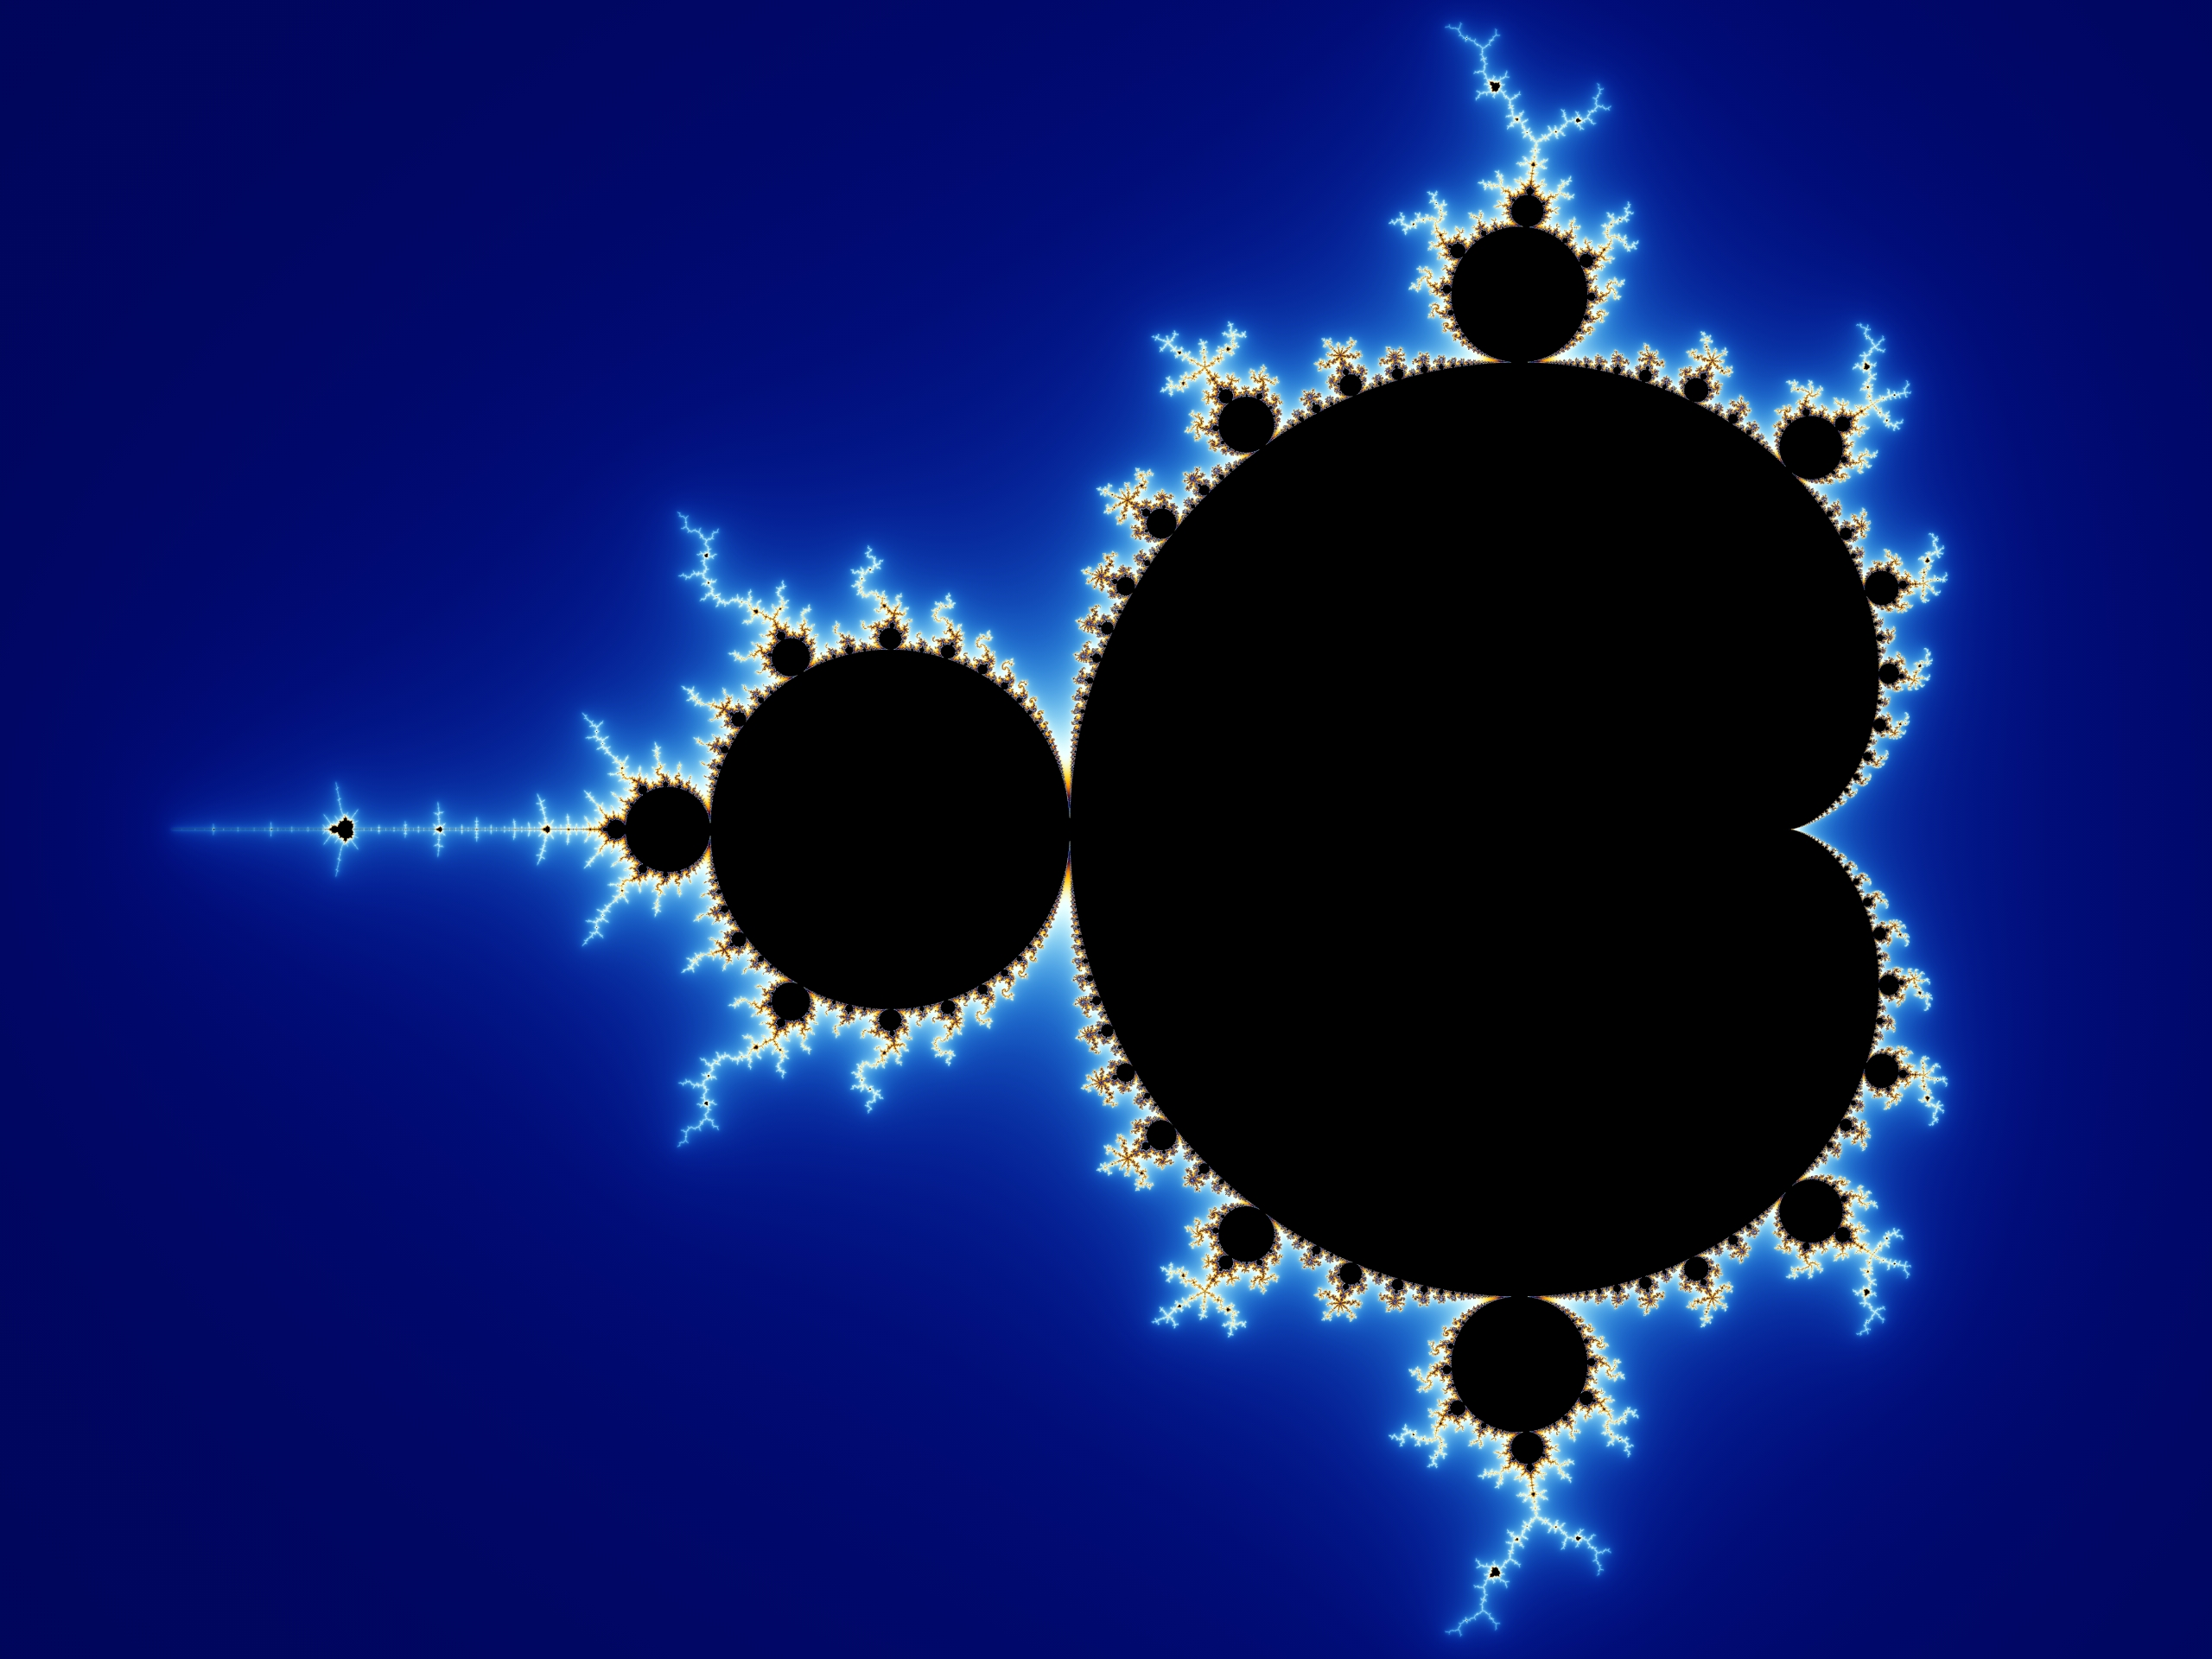
\includegraphics[width=0.8\textwidth]{images/sec-5/mandelbrot}
%     \end{center}
%     \caption[The Mandelbrot fractal]{Image of a Mandelbrot set with a
%         continuously coloured environment. Each pixel corresponds to a point $c$
%         in the complex plane, and its colour depends the number of iterations
%         $n$ before the relation diverges.}
%     \label{fig:mandelbrot}
% \end{figure}
% 
% \note{Introduce the (?) operator, talk about what divergence is, why it is bad,
% etc.}
% 
% How can we express this computation in a language without iteration? Instead, we
% use generative (meta-programming) techniques to express the recurrence relation.
% Begin by first defining a single step of the relation for a single point in the
% plane. For each point $c$ we keep a pair of elements $\left( z, n \right)$ where
% $z$ is the current value of the relation and $n$ is the iteration that
% divergence occurred at, or the current iteration otherwise.
% %
% \begin{lstlisting}[style=haskell]
% iter :: Exp Complex -> Exp (Complex, Int) -> Exp (Complex, Int)
% iter c z_n = ...
% \end{lstlisting}
% %
% This computes the next value of the polynomial $z_{n+1}$ as well as the number
% of iterations $n$ if the element has not diverged, otherwise returns the value
% and iteration count (at divergence) unchanged. We then lift this to the
% Accelerate array language by applying the operation at all points in the plane
% \texttt{cs}:
% %
% \begin{lstlisting}[style=haskell,firstnumber=last]
% step :: Acc (Array DIM2 (Complex,Int)) -> Acc (Array DIM2 (Complex,Int))
% step = A.zipWith iter cs
% \end{lstlisting}
% %
% Note that we have to apply the function even to elements that have already
% diverged. This wastes work but means that there is less SIMD divergence because
% we still do the same thing to every element at every iteration. Here the ``same
% thing'' does imply a small amount if divergence, between elements that have
% already diverged and those that have not, but w
% 
% We can then use
% standard Haskell to unroll the loop a \emph{fixed} number of times, which
% completes the Mandelbrot set calculation:
% %
% \begin{lstlisting}[style=haskell,firstnumber=last]
% mandelbrot :: Acc (Array DIM2 (Complex,Int)) -> Acc (Array DIM2 (Complex,Int))
% mandelbrot = foldr ($) zs0 (replicate depth step)
% \end{lstlisting}
% %
% Here \texttt{foldr} and \texttt{replicate} come from the standard Haskell
% prelude, and \texttt{depth} is the maximum iteration count of the relation.
% 
% This correctly computes the Mandelbrot set, but is outrageously slow because it
% must read and write the values $z$ and $n$ to memory at each step of the
% computation, rather than keeping these values in registers, computing the entire
% recurrence relation and storing only the final result to memory. Later, we will
% see how the technique of \emph{array fusion} (\S\ref{sec:fusion}) can be used to
% eliminate this intermediate memory traffic by combining the \emph{depth}
% applications of the collective operation \texttt{zipWith iter} into a single
% operation containing \texttt{depth} instances of the scalar function
% \texttt{iter}, which does not require us to write the intermediate values to
% memory. However, doing this we uncover an embarrassing secret: \emph{a C
% compiler does not compile C code}, it compiles \emph{idiomatic} C code. While
% combining the sequence of collective operations into a single collective
% operation containing a sequence of scalar operations produces faster code due to
% reduced memory traffic, it is still far from optimal.
% 
% The problem is that fusing the collective operations in this way does not
% preserve the iteration structure of the recurrence relation, and the loop is
% completely unrolled in the single fused operation. We can introduce scalar loops
% by looking for the following pattern:
% %
% \begin{lstlisting}[style=Haskell,numbers=none,mathescape]
% %\bf$\langle$ loop introduction $\rangle$%
%     let x =
%         let y = e1
%         in e2
%     in e3
%     $\mapsto$
%     iterate[2] (\y -> e2) e1            %\rm if \texttt{e2} $\equiv$ \texttt{e3}%
% \end{lstlisting}
% %
% The nested bindings are replaced with an explicit scalar value iteration
% structure, where the expression \texttt{e2} is repeated twice with the initial
% value \texttt{e1}. Similarly, loops can be joined:
% %
% \begin{lstlisting}[style=Haskell,numbers=none,mathescape]
% %\bf$\langle$ loop joining $\rangle$%
%     let x = iterate[n] f e1
%     in e2
%     $\mapsto$
%     iterate[n+1] f e1                   %\rm if the body of \texttt{f} $\equiv$ \texttt{e2}%
% \end{lstlisting}
% %
% Recovering scalar loops in this way enables a backend to generate explicit loops
% in its target language, such as CUDA, and ultimately results in higher
% performance code. In future, it would be beneficial to augment it with related
% loop optimisations such as loop invariant code motion in the frontend and
% lower-level code generation optimisations in a backend.


\subsection{Redundancy Elimination}
\label{sec:redundancy_elimination}

The optimisations in this section deal with the elimination of redundant
computations. These procedures almost always improve the performance of the code
they are applied to.

\subsubsection{Sharing Observation}

\marginnote{describe why this is difficult for deeply embedded DSLs. approaches
other than sharing}
As described in section~\derp, operations of the embedded language do not
directly issue computations; instead, they build term trees that represent
the embedded computation. These term trees use \indexe{higher-order abstract
syntax} (HOAS)\index{HOAS|see{higher-order abstract syntax}}
to embed function-valued scalar expressions as well as typeclass overloading to
reflect arithmetic expressions.

The HOAS representation, while convenient for the human reader, is awkward for
program transformations as it complicates looking under lambdas --- i.e.,
inspecting and manipulating the bodies of function abstractions. The frontend
converts HOAS terms into a \emph{nameless de Bruijn representation} \index{de
Bruijn} in the style of \citet{Altenkirch:2003kz}, using GADTs \cite{Jones:2006}
and type families \cite{Chakravarty:2005a,Schrijvers:2008} to preserve the
embedded program's type information. The type-preserving HOAS to de Bruijn
conversion is described elsewhere
\cite{Atkey:2009,Chakravarty:2009uo,McDonell:2013wi}.

Together with the conversion to a nameless representation, we recover the
sharing introduced by \texttt{let}-bound subterms in the embedded program. For
example, consider:
%
\begin{lstlisting}[style=Haskell]
let ys = map f xs
in  zipWith g ys ys
\end{lstlisting}
%
If we do not take care, the expression will be inefficiently translated as:
%
\begin{lstlisting}[style=Haskell]
zipWith g (map f xs) (map f xs)
\end{lstlisting}
%
because the straightforward evaluation of the surface language program results
in a complete unfolding of the expression into embedded language terms. To
recover sharing, we user a variant of Gill's technique \cite{Gill:2009dx}; in
contrast to this work, we preserve types and produce a nested term with minimal
flattening, instead of a graph. A complete treatment of the sharing recovery
algorithm appears in \derp; in brief it proceeds in the following phases:

\paragraph{Phase 1: Build the occurrence map}

A top-down traversal of the AST that computes a map from AST nodes to the number
of occurrences of that node in the overall program; an occurrence count of two
or more indicates sharing. During computation of the occurrences, the tree is
annotated with the \indexe{stable name} \cite{Jones:2000} of that node, and all
but the first occurrence of shared subtrees are pruned and replaced with
variable bindings. Note that to avoid completely unfolding the embedded
expression, we do not descend into subterms that have been encountered
previously, making the complexity of sharing observation proportional to the
number of nodes in the tree \emph{with} sharing.

As it is based on stable names this phase of the algorithm is impure and,
strictly speaking, because of this it is not deterministic. The stable name API
does not guarantee completeness,\footnote{For two stable names \lstinline{sn1}
and \lstinline{sn2}, if \lstinline{sn1 == sn2} then the two stable names were
created from the same object. However, the reverse is not necessarily true; if
the two stable names are not equal the objects they come from may still be
equal.} which means that we may miss some equalities which implies we fail to
discover some sharing. Luckily, sharing does not affect the denotational meaning
of the program, and hence a lack of sharing does not compromise denotational
correctness.


\paragraph{Phase 2: Determine scope and inject sharing information}

A bottom-up traversal that determines the scope for every binding to be
introduced to share a subterm. It uses the occurrence map to determine, for
every shared subtree, the meet of all the shared subtree occurrences --- the
lowest AST node at which the binding for the subterm can be placed.

\paragraph{Phase 3: Convert to de Bruijn form}

Finally, the AST with environment layout and sharing information can be
converted into de Bruijn form while incorporating sharing by introducing
appropriate \texttt{let} bindings.\\

\noindent
We now correctly observe the sharing of our motivating example, producing the
following (simplified) core language term:
%
\marginnote{this is weird: mixes core/library language terms}
\begin{lstlisting}[style=Haskell,numbers=none,mathescape]
%\bf$\langle$ sharing observation $\rangle$%
    let ys = map f xs in zipWith g ys ys
      $\mapsto$
      Alet (Map f xs)
           (ZipWith g (Var ZeroIdx) (Var ZeroIdx))
\end{lstlisting}


\subsubsection{Common Subexpression Elimination}
\label{sec:cse}

\emph{Common subexpression elimination} finds computations that are performed at
least twice on a given execution path and eliminates the second and later
occurrences, replacing them with uses of saved values. The current
implementation performs a simplified version of common subexpression, where we
look for expressions of the form:
%
\begin{lstlisting}[style=Haskell,numbers=none]
%\bf$\langle$ common subexpression elimination $\rangle$% let x = e1 in [x/e1]e2
\end{lstlisting}
%
and replace all occurrences of \texttt{e1} in \texttt{e2} with \texttt{x}. This
is not complete full redundancy analysis, but is good enough to catch some
cases.%\footnote{\url{http://hackage.haskell.org/trac/ghc/ticket/701}}

While it may seem that common subexpression elimination is always worthwhile, as
it reduces the number of arithmetic operations performed, this is not
necessarily advantageous. The simplest case in which it may not be desirable is
if it causes a register to be occupied for a long time in order to hold the
shared expression's value, which hence reduces the number of registers available
for other uses. Even worse is if the value has to be spilled to memory because
there are insufficient registers available. We sidestep this tricky and
target-dependent issue by, for now, simply ignoring it.


% \subsubsection{derp Loop-Recovery [DEPRECATED]}
% \subsubsection{derp Loop-Invariant Code Motion [TODO]}


\section{Array Fusion}
\label{sec:fusion}

Fusion or deforestation is a term used to describe techniques for having a
compiler automatically eliminate intermediate data structures in a computation.
For example, to compute the sum of squares of all integers from one to a given
number in Haskell~\cite{Haskell:1998}, I could write:
%
\begin{lstlisting}[style=haskell]
sum_of_squares :: Int -> Int
sum_of_squares n
    = sum                       -- add all numbers in the list
    $ map (\x -> x * x)         -- traverse list doubling each element
    $ enumFromTo 1 n            -- generate list of numbers [1..n]
\end{lstlisting}
%
but while the meaning of the program is clear, it is inefficient, as this code
produces two intermediate lists of numbers which requires $O(n)$ space and
associated memory pressure to manipulate. Instead, one could write the program
as a single tail-recursive loop as such:
%
\begin{lstlisting}[style=haskell]
sum_of_squares :: Int -> Int
sum_of_squares n = go 1 0
  where
    go i acc | i > n     = acc                   -- return final tally
             | otherwise = go (i+1) (acc + i*i)  -- add to accumulator and step to next element
\end{lstlisting}
%
The second program is much more efficient than the first, because it does not
involve the production of any intermediate lists and executes is constant space.
Unfortunately, the clarity of the original program has been lost. What we
\emph{really} want is to write the first program, and have the compiler
\emph{automatically} transform it into the second, or something morally
equivalent.

This example also demonstrates a subtle behavioural tendency of optimising
program transformations: while the second (target) program does not produce any
intermediate data structures as desired, we can no longer interpret the program
as a sequence of combinators. This observation is critical if the combinators
represent \emph{collective} operations as they do in Accelerate: while the
second program compiles to an efficient scalar loop, its \emph{parallel}
interpretation has been lost.


\subsection{Related Work}

The desire to program in a functional style while still achieving the
performance level of an imperative language has been around for as long as
functional programming itself. This section briefly summarises some of the key
milestones in the history of deforestation as a compiler optimisation that
influences this work.

\subsubsection{Deforestation}

% blugh blurgh
Inspired by earlier work in \texttt{fold/unfold} methods (for example
\citet{Burstall:1977kl}), Philip Wadler set out to develop a technique that
would \emph{automatically} remove intermediate structures from functional
programs, a technique he (later) dubbed \indexe{deforestation}
\cite{Wadler:1981hy,Wadler:1990ix}.

The method identifies a core set of list operators that can be used to express a
large class of computations: \texttt{map}, \texttt{reduce} and
\texttt{generate} (the latter being similar in spirit to \texttt{foldr} and
\texttt{unfoldr} respectively), together with a collection of rewrite rules that
apply to combinations of these operators. These rules identify specific patterns
of list operators that create then consume intermediate lists, then merges these
operations to avoid the intermediary.

\paragraph{Advantages}
\begin{itemize}
    \item Automatic: does not require programmer input, and therefore suitable
        for integration to a compiler.

    \item Source-to-source: all transformations take valid programs in the
        source language and output (faster) valid programs in the source
        language. This makes the output of deforestation easy to integrate as
        part of a compiler pipeline.

    \item Simple: each rule is easy to understand and obviously correct.
\end{itemize}

\paragraph{Disadvantages}
\begin{itemize}
    \item Each optimisation requires a separate transformation rule. If we want
        to add new list operators, we need to add a new rule for each
        combination of the new operator with each existing operator. This does
        not scale.

    \item Limited: many computations can not be expressed in terms of these
        three operations, so the framework can not eliminate intermediate lists
        in these case. \marginnote{check this, c.f. adv of foldr/build}
\end{itemize}


\subsubsection{foldr/build}

Building upon the original deforestation algorithm, Andy
Gill's doctoral thesis introduces another approach to deforestation known as
\indexe{foldr/build fusion} \cite{Gill:1996tf,Gill:1993de}.
% This techniques performs a range of optimisations as broad as previous
% approaches the listless transformer \cite{Wadler:1984ia,Wadler:2005iw} while
% addressing their drawbacks.
Like the deforestation algorithm, \texttt{foldr/build} fusion is a rule-based
source-to-source transformation. In fact, it is based on a single rule:
%
\begin{lstlisting}[style=Haskell,numbers=none,mathescape,caption={The \texttt{foldr/build} transformation}]
%\bf$\langle$ foldr/build fusion $\rangle$% forall g k z. foldr k z (build g) $\mapsto$ g k z

build :: (forall b. (a -> b -> b) -> b -> b) -> [a]
foldr :: (a -> b -> b) -> b -> [a] -> b
\end{lstlisting}

The idea is to think of \texttt{build} as a function that constructs a list, and
\texttt{foldr} as a list consumer. Because of this uniform treatment of lists as
\emph{complete objects}, rather than being composed of many individual
constructor cells, we can have a single \texttt{foldr/build} rule, which is
analogous to standard case reduction rules, but instead of removing a single
constructor removes the \emph{entire data structure}. This method became the
first non-trivial deforestation system to be included as an active part of a
production quality functional language compiler.

\paragraph{Advantages}
\begin{itemize}
    \item Simple, automatic, source-to-source transformation.

%    \item No limitation on inputs: \texttt{foldr/build} fusion operates over the
%        entire Haskell language. When a list is produced without using
%        \texttt{build} or consumed without using \texttt{foldr}, the
%        deforestation scheme is not hampered and simply leaves the list intact.

    \item Single rule: unlike the original deforestation algorithm, a single
        rule suffices. When new list operations are added, so long as they cane
        be expressed in terms of \texttt{foldr} and \texttt{build}, the
        transformation will apply; there is no need to consider all combinations
        with the existing operations.
\end{itemize}

\paragraph{Disadvantages}
\begin{itemize}
    \item The transformation can not handle functions that use accumulators,
        such as \texttt{foldl}, or consume multiple inputs, such as
        \texttt{zip}.

    \item Operations that do not produce lists using \texttt{build} or consume
        them using \texttt{foldr} will not have the intermediate list
        eliminated.
\end{itemize}


\subsubsection{Stream Fusion}

Following Gill's work, a whole cottage industry of new deforestation approaches
appeared with the goal of covering the cases left out by \texttt{foldr/build}.
Most of that work was theoretical, a lot of it was based on category theory, and
almost none of it had any impact in practice. Unlike those systems of the prior
two decades, \indexe{stream fusion} \cite{Coutts:2007} succeeded in this goal and
at the same time stayed simple and useful in practice.

Stream fusion has a similar structure to \texttt{foldr/build}: a single rule
eliminates matching pairs of constructor and destructor, and operations need to
be expressed in terms of these constructors:
%
\begin{lstlisting}[style=Haskell,numbers=none,mathescape,caption={The \emph{stream fusion} transformation}]
%\bf$\langle$ stream fusion $\rangle$% forall s. stream (unstream s) $\mapsto$ s

stream   :: [a] -> Stream a
unstream :: Stream a -> [a]

data Stream a = exists s. Stream (s -> Step a s) s
data Step a s = Done
              | Yield a s           -- produce a value and new state
              | Skip s              -- update the state without producing a value
\end{lstlisting}

Streams have some abstract state and a \emph{stepper} function that advances the
stream from one state to the next, possibly yielding a new value. The
\texttt{stream} constructor \texttt{Yield}s values from its input until it runs
out, and the \texttt{unstream} destructor build a list by consuming its input
stream until encountering \texttt{Done}, discarding \texttt{Skip}s along the
way. Applying the rule to keep the computation in the non-recursive
\texttt{Stream} formulation allows the compiler to aggressively apply standard
optimisation techniques.

\paragraph{Advantages}
\begin{itemize}
    \item Preserves the nice properties of \texttt{foldr/build} fusion.
    \item Adds supports operations with accumulators and multiple inputs.
\end{itemize}

% \paragraph{Disadvantages}
%
% \begin{itemize}
%     \item None, really\ldots? Requires a highly optimising compiler?
% \end{itemize}


\subsubsection{Delayed Arrays}

The previous fusion transformations are based on the idea of expressing
computations in terms of a builder and consumer function, and then having the
compiler identify and remove adjacent constructor/destructor pairs. In contrast,
the Repa \cite{Keller:2010} library uses a functional representation of
\indexe{delayed arrays} that instead \emph{avoids} creating unnecessary
intermediate structures, rather than relying on a subsequent fusion
transformation to remove them.

\begin{lstlisting}[style=Haskell,numbers=none,caption={Repa-1 style array definition},label={lst:repa_arrays}]
data Array sh e = Manifest sh (Vector e)    -- unboxed data
                | Delayed  sh (sh -> e)     -- array shape and indexing function
\end{lstlisting}

The key principle of the design is to avoid generating an explicit
(\texttt{Manifest}) representation of intermediate arrays that can instead be
represented as the original array combined with an index-space transformation
function.

% Repa retains the functional programming style by exposing an interface of
% collective operations over arrays --- such as maps, folds, and permutations ---
% instead of the imperative style of reading and writing individual array
% elements.

\paragraph{Advantages}
\begin{itemize}
    \item Explicitly avoids intermediate structures by design, rather than
        relying on potentially fragile post hoc compiler transformations.
\end{itemize}

\paragraph{Disadvantages}
\begin{itemize}
    \item Requires the user to explicitly state when arrays should be computed
        (made manifest), else performance suffers due to redundant computation.
\end{itemize}



\subsection{Accelerate Arrays, Accelerated}

In the previous section, we briefly reviewed related work on fusion in
functional languages. From this we can state some aims for a fusion
transformation that is to be developed for the Accelerate language:

\begin{itemize}
    \item The transformation must retain the combinator-based interpretation of
        the program, which is necessary to support execution on parallel
        architectures such as CUDA.

    \item Fuse everything: The transformation should cover all Accelerate
        operations, and not be limited to common special cases such as
        \texttt{map/map} and \texttt{map/fold}.

    \item Source-to-source: The fusion transformation should take valid source
        (or core) programs and return valid programs in the same representation.
        This is important for integration into existing phases of the compilation
        pipeline and multiple-backend architecture. Tangentially, this forces
        adherence to the first requirement.

    \item Have a constant number of rewrite rules: Adding new terms to the core
        language should not require adding new rules for each combination of the
        new operator to the existing operations. Furthermore, adding new
        combinators should be relatively easy to integrate into the fusion
        schema.
\end{itemize}
%
Looking at the historical progression of the fusion transformation in a
different way helps inform the design requirements for the Accelerate fusion
algorithm:
%
\begin{itemize}
    \item Wadler's deforestation technique applied fusion rules directly to
        source language terms, requiring a number of rewrite rules quadratic in
        the number of operations that are to be fused.

    \item Gill's \texttt{foldr/build} instead requires a constant number of
        rewrite rules because it first expressed the source language operations
        in terms of more primitive operations --- \texttt{foldr} and
        \texttt{build} --- and then applied the transformation to this reduced
        set.

    \item However, \texttt{foldr/build} fails to capture all cases because its
        core combinators are not expressive enough. This infelicity is addressed
        by both stream fusion and delayed arrays, which fuse all operations
        using a constant set of rules by having a sufficiently expressive
        intermediate form to be able to define all operations in their
        respective libraries.
\end{itemize}

The task, then, is to identify this reduced set of operations within which we
can encode all Accelerate array operations which we would like to be subject to
fusion, and then develop a (hopefully) constant number of rules to fuse these
intermediate forms into, followed by their translation back into core language
operations. We shall return to this list of design criteria when we discuss the
results generated by the optimisation pass. For now, we turn the discussion
towards implementation.

\subsection{Of Predators and Prey}

The classic array fusion example is that of vector dot product:
%
%    label={lst:dotp},
%    caption={Vector dot product in Accelerate}]
\begin{lstlisting}[style=haskell]
dotp :: Acc (Vector Float) -> Acc (Vector Float) -> Acc (Scalar Float)
dotp xs ys = fold (+) 0 (zipWith (*) xs ys)
\end{lstlisting}
%
Ideally, our fusion system will translate this into a single collective
operation, in much the same way as what a human would write if working directly
in a low-level language such as C or CUDA. Before we get to the meat of the
topic, we must classify the existing set of core language operations, and define
how we wish the deforester to handle each class of operations.

\subsubsection{Producers}

We begin by defining \emph{producers}\index{producer} as the class of operations
that, given a set of zero or more input arrays, produce a single element for the
output array by manipulating a \emph{single} element from each input array. This
can be further classified along several dimensions: value transformers such as
\texttt{map} and \texttt{zipWith} apply a scalar function to each element of
their input array(s). On the other hand, index space transformations such as
\texttt{backpermute}, \texttt{slice} and \texttt{replicate}, in effect rearrange
elements of the input array without changing the array values. In either case,
each output array element is calculated independently of all other array
elements. In fact, at the expense of any specific behavioural knowledge of the
collective operation, \texttt{generate}, combined with the scalar array
indexing operator \texttt{(!)}, is the most general array production mechanism,
and is capable of expressing all other producer operations.

Since all producers operate on an element of the array independent of all other
elements, at a first approximation it is reasonable to propose that our fusion
system should be able to combine arbitrary sequences of producers into a single
operation.


\subsubsection{Consumers}

We define \emph{consumers}\index{consumer} as collective operations that compute
elements of their output array using \emph{multiple} elements of their input
array(s). Since such collective operations often have particular parallel
interpretations which we wish to preserve, we will always force these operations
to be computed rather than attempting to fuse them with later stages of the
computation.

Depending on the type of collective operation, we may be able to fuse the inputs
directly into the consumer: \texttt{fold*}, \texttt{scan*}\footnote{A parallel
scan implementation typically splits the input array into contiguous chunks over
the available processing elements and requires two passes over the data. The
first phase computes a partial block sum and then the second phase distributes
these partial sums to each processing element to use as a carry-in value.
Nevertheless, it is possible for an implementation to consume the fusion
material in the first phase only.} and \texttt{permute} read each input array
element once, and so are good candidates for fusing the input arrays directly
into the collective operation step.

On the other hand, because \texttt{stencil*} operations apply the stencil
function with access to all elements within a local neighbourhood of the focus
point/array element, each element of the input array may be read multiple times.
Thus, stencil operations first fully compute their input array(s), and then
fully evaluate their output arrays.


\subsubsection{Flow Control}

The remaining constructors of the Accelerate array term tree express environment
and control flow operations. These include conditional statements
(\texttt{|?}), introduction of constant array data (\texttt{use} and
\texttt{unit}), array tupling and projection, pipelining (\texttt{>->}) and
environment bindings. While there may be some opportunity here --- moving array
conditionals into scalar expressions or eliminating the aggregate tupling
structure in an attempt to expose further opportunities for fusion --- we
currently do not attempt to fuse past these points of the expression. In
general, we will not attempt to fuse past control-flow nodes of the expression.

We note that the key disadvantage of the Repa delayed array representation was
that it failed to capture array sharing, leading to excessive recomputation and
corresponding loss of performance if the user did not explicitly demand results
to be computed at the correct locations in the program. However, because
Accelerate is a \emph{deeply-embedded} language with an explicit sharing
observation algorithm, these program locations where data must be computed to
avoid duplicated work have been reified as part of the term tree. Any
\texttt{let}-bound array expression implies sharing and so the fusion
transformation should not fuse these expressions else it will introduce
duplicate work. Thus, we neatly sidestep the main infelicity of delayed arrays.


\subsubsection{Conclusion}

In summary, the primary goals of the deforester is that it should be able to
fuse arbitrary sequences of producer operations into a single producer term,
and, excepting \texttt{stencil}, fuse producers directly into consumers
outputting a consumer term. Additionally, we do not fuse into
\texttt{let}-bindings in order to avoid work duplication.

Implicit in the above taxonomy, what we are discriminating against is the
collective behaviour of the array \emph{elements}. This is a key insight:
whatever reduced set of intermediate form(s) we choose, these operations will
describe the transformation of individual elements, and based on a given
collection of scalar operations, we must be able to reconstruct an appropriate
collective operation form.

\begin{lstlisting}[
    style=haskell,
    numbers=none,
    float=tp,
    label={lst:operations},
    caption={[Core Accelerate array operations] Summary of Accelerate's core
        collective array operations, omitting \texttt{Shape} and \texttt{Elt}
        class constraints for brevity. In addition, there are other flavours of
        folds and scans as well as segmented versions of these.
        \note{integrate with body text}}]
%\makebox[\textwidth]{\rm\bf Producers}%

map         :: (Exp a -> Exp b) -> Acc (Array sh a) -> Acc (Array sh b)       %\rm map a function over an array%
zipWith     :: (Exp a -> Exp b -> Exp c) -> Acc (Array sh a)                  %\rm apply funciton to\ldots%
            -> Acc (Array sh b) -> Acc (Array sh c)                           %\rm \ldots a pair of arrays%

backpermute :: Exp sh' -> (Exp sh' -> Exp sh) -> Acc (Array sh a)             %\rm backwards permutation%
            -> Acc (Array sh' e)
replicate   :: Slice slix                                                     %\rm extend array across\ldots%
            => Exp slix -> Acc (Array (SliceShape slix) e)                    %\rm \ldots new dimensions%
            -> Acc (Array (FullShape slix) e)
slice       :: Slice slix                                                     %\rm remove existing dimensions%
            => Acc (Array (FullShape  slix) e) -> Exp slix
            -> Acc (Array (SliceShape slix) e)

generate    :: Exp sh -> (Exp sh -> Exp a) -> Acc (Array sh a)                %\rm array from index mapping%

%\makebox[\textwidth]{\rm\bf Consumers}%

fold        :: (Exp a -> Exp a -> Exp a) -> Exp a -> Acc (Array (sh:.Int) a)  %\rm tree reduction along\ldots%
            -> Acc (Array sh a)                                               %\rm \ldots innermost dimension%
scan{l,r}   :: (Exp a -> Exp a -> Exp a) -> Exp a -> Acc (Vector a)           %\rm left-to-right or right-to-left%
            -> Acc (Vector a)                                                 %\rm \ldots vector pre-scan%
permute     :: (Exp a -> Exp a -> Exp a) -> Acc (Array sh' a)                 %\rm forward permutation%
            -> (Exp sh -> Exp sh') -> Acc (Array sh a) -> Acc (Array sh' a)
stencil     :: Stencil sh a stencil => (stencil -> Exp b) -> Boundary a       %\rm map a function with local\ldots%
            -> Acc (Array sh a) -> Acc (Array sh b)                           %\rm \ldots neighbourhood context%
\end{lstlisting}

\subsection{The Elements of Style}
\label{sec:elements_of_style}

We begin the discussion of how to implement fusion in Accelerate through the use
of a few motivating examples. We start with fusion of producer functions, of
which we would like to fuse arbitrary sequences into a single operation. We have
already mentioned some prototypical producer fusion rules, such as the classic
\texttt{map/map} rule, which combines two value transformation operations into a
single step:
%
\begin{lstlisting}[style=haskell,numbers=none,mathescape]
%\bf$\langle$ RULE: map/map $\rangle$%
    map f (map g arr) $\mapsto$ map (f . g) arr
\end{lstlisting}
%
By extension, we can similarly combine two index space transformations into a
single step:
%
\begin{lstlisting}[style=haskell,numbers=none,mathescape]
%\bf$\langle$ RULE: backpermute/backpermute $\rangle$%
    backpermute sh p (backpermute _ q arr) $\mapsto$ backpermute sh (q . p) arr
\end{lstlisting}

We observe that, as mentioned in the concluding remarks of the previous section,
these rules are described by composing the scalar components of the collective
operation. But what about for combinations of index/value space or value/index
space transformations? This informs the first choice of intermediate combinator:
an array transformation step with embedded index \emph{and} value space
transformations. In fact, we shall add this to the set of core language
operations:
%
\begin{lstlisting}[style=haskell,numbers=none]
Transform :: (Elt a, Elt b, Shape sh, Shape sh')
          => PreExp     acc aenv sh'                    -- dimension of the result
          -> PreFun     acc aenv (sh' -> sh)            -- backward permutation indexing function
          -> PreFun     acc aenv (a   -> b)             -- function to apply at each element
          ->            acc aenv (Array sh  a)          -- source array
          -> PreOpenAcc acc aenv (Array sh' b)
\end{lstlisting}
%
And a rule to combine two operations of this form:
%
\begin{lstlisting}[style=haskell,numbers=none,mathescape]
%\bf$\langle$ RULE: transform/transform $\rangle$%
    transform sh p1 f1 (transform _ p2 f2 arr) $\mapsto$ transform sh (p2 . p1) (f1 . f2) arr
\end{lstlisting}
%
Finally, we need to know how to map our original \texttt{map} and
\texttt{backpermute} in terms of this new constructor:
%
\begin{lstlisting}[style=haskell,numbers=none,mathescape]
map f arr            $\mapsto$ transform (shape arr) id f arr
backpermute sh p arr $\mapsto$ transform sh p id arr
\end{lstlisting}
%
Oops! In order to recast a \texttt{map} into the more general
\texttt{transform}, we needed to take the \texttt{shape} of the input array, but
to do that we have just introduced duplicated work as the arbitrarily complex
\texttt{arr} is now used twice in the new term. Disaster! This will not do, so
let us first \texttt{let}-bind the input array expression and refer to it:
%
\begin{lstlisting}[style=haskell,numbers=none,mathescape]
map f arr $\mapsto$ let v = arr
             in  transform (shape v) id f v
\end{lstlisting}
%
And this correctly maintains the complexity of the original term. The
\texttt{map/map} fusion rule now proceeds as follows:
%
\begin{lstlisting}[style=haskell,numbers=none,mathescape]
map f (map g arr) $\mapsto$ map f (let v = arr in transform (shape v) id g v)
                  $\mapsto$ ??
\end{lstlisting}
%
And once again we are stuck. One of our original premises is that we should not
fuse past \texttt{let} bindings so as to avoid the problem of duplicated work
endemic to delayed array fusion in Repa. And so it is in this case: \texttt{v}
here represents a multiply-used expression which we must not inline. So herein
lies the second device required for our intermediate combinators: we need to
make a distinction between sharing in the source program and sharing introduced
as part of the fusion transformation.

Armed with a strategy to deal with an index or value transformation applied to
an array (as we shall see, \texttt{slice} and \texttt{replicate} can be
represented in terms of \texttt{backpermute}), we now need to develop a way to
deal with multiple arrays (\texttt{zipWith}), which historically speaking has
proved to be rather challenging for fusion systems, as well as the
\texttt{generate} function which takes no explicit input arrays. Since
\texttt{generate} has no input arrays, we only need to consider a single rule:
%
\begin{lstlisting}[style=haskell,numbers=none,mathescape]
%\bf$\langle$ RULE: generate/transform $\rangle$%
    transform sh p f (generate _ g) $\mapsto$ generate sh (f . g . p)
\end{lstlisting}
%
Previously we mentioned that \texttt{generate} is the most general form of
producer; we will exploit that fact here to define \texttt{zipWith} in
terms of \texttt{generate}, and so fuse the operation without needing to
generalise our other combinators for multiple input arrays:
%
\begin{lstlisting}[style=haskell,numbers=none,mathescape]
zipWith f xs ys $\mapsto$ let v1 = xs
                       v0 = ys
                   in generate (shape v1 `intersect` shape v0)
                               (\ix -> f (v1!ix) (v0!ix))
\end{lstlisting}
%
Where again we needed to \texttt{let}-bind the input arrays of \texttt{zipWith}
in order to avoid work duplication, and \texttt{(!)} indexes an array at the
given index. These two rules suggest that our approach to fusion will tend
towards fusing producer functions into a \texttt{generate} node. In fact, we
could also formulate \texttt{map} and \texttt{backpermute} in terms of
\texttt{generate} as well, which is the approach taken by Repa delayed arrays
(listing~\ref{lst:repa_arrays}). However, we should be cautious; being the most
general combinator, \texttt{generate} lacks any specific knowledge of the
collective behaviour of the expression, so later frontend analysis or a specific
backend implementation may lose opportunities for optimisation.

% TLM: hoom\ldots\ actually because I couldn't figure out how to do it.
\marginnote{additional design constraints?}
Finally, we should make a note about fusing consumer functions. Since Accelerate
supports multiple backends, it is particularly important that we retain the
property of the fusion algorithm being a source-to-source transformation. This
allows fusion to be easily integrated with other parts of the compiler --- which
we may have no control over --- and potentially simplifies the implementation of
a backend by being able to ignore producer/consumer fusion.


\subsection{Environment Manipulation}
\label{sec:environment_manipulation}

As discovered in the previous section, as part of the fusion transformation of
recasting terms we often need to lift array valued inputs to be
\texttt{let}-bound at higher points to avoid work duplication, but at the same
time we can not immediately add these bindings to the output term because they
will interfere with further fusion steps. We need to collect these extra
bindings separately from the main term, and only add them to the output once we
encounter a node that forces the computation, such as a consumer. Furthermore,
we must ensure we correctly track the types of the environments between the
fused terms and the collected \texttt{let}-bindings.

The following is a heterogeneous snoc-list of array terms that witnesses how an
array environment is extended by the application of these operations:
%
\begin{lstlisting}[
    style=haskell,
    label={lst:Extend},
    caption={Extending an array environment}]
data Extend aenv aenv' where
    BaseEnv ::                                                                Extend aenv aenv
    PushEnv :: Arrays a => Extend aenv aenv' -> PreOpenAcc OpenAcc aenv' a -> Extend aenv (aenv', a)
\end{lstlisting}
%
In the style of the de Bruijn indices used for projecting environment variables
(\S\derp), \texttt{Extend} uses an inductive notion of tuples as heterogeneous
\emph{snoc} lists. In contrast to environment indices, the base case does not
refer to an empty environment, but instead the arbitrary environment to which we
are extending. This witnesses how to connect the environment of the original
term which we are currently deforesting to the new terms being output by the
deforester. We will refer to \texttt{aenv} as the external environment type, and
\texttt{aenv'} as the internal environment type. Binding these expressions to
the term output by the deforester yields a completed term of the correct type.
%
\begin{lstlisting}[style=haskell]
bind :: Arrays a
     => Extend aenv aenv'               -- collection of additional environment bindings
     -> PreOpenAcc OpenAcc aenv' a      -- term output by the deforester
     -> PreOpenAcc OpenAcc aenv  a
bind BaseEnv         = id
bind (PushEnv env a) = bind env . Alet (OpenAcc a) . OpenAcc
\end{lstlisting}


\subsection{Implementing Fusion}

% The basic strategy of the fusion process is to traverse the array expression
% bottom-up, and then depending on the type of node encountered proceed as
% follows:
% %
% \begin{itemize}
%     \item \textbf{Producer:} Convert the node into the reduced form on which the
%         fusion rules will be applied as outlined previously
%         (\S\ref{sec:node_taxonomy}), which will be either
%         \texttt{transform}-like or \texttt{generate}-like in appearance.
%         Additional \texttt{let}-bindings introduced by the term recasting are
%         tracked separately via an \texttt{Extend}ed environment list, which
%         enables successive producer nodes to be fused together without
%         interference.
% 
%     \item \textbf{Consumer:} Force the node to be evaluated by adding the input
%         node and \texttt{bind}ing the \texttt{Extend}ed environment to the
%         output term together with the current consumer node. We belay the
%         discussion of how best to represent producer/consumer fusion in the term
%         tree.
% 
%     \item \textbf{Control:} Nodes that represent control flow or array injection
%         are largely left intact. Later, we will discuss when it is advantageous
%         to break the rules and fuse \texttt{let}-bound term directly into the
%         body expression.
% 
% \end{itemize}

% \note{These previous bullet points can be integrated as actual text.
% Following the below, talk about the implementation of delay; what we do at
% producer/consumer/control nodes.}

Finally, we reach the question of how to implement the fusion optimisation. As
evidenced in the preceding sections,
%As embodied in the previous work, and indicated by the preceding sections,
fusion is expressed as a set of transformations between terms. We could attempt
to do this statically, at compile time using rewrite rules \cite{Jones:2001wm},
but doing so requires the consumer to ``see'' the producer function. While this
would work in some cases, it may be difficult for the programmer to predict
whether or not the optimisation will take place. The killer, however, is that
Accelerate is a meta-programming language that allows computations to be built
programmatically at [program] runtime, a domain in which rewrite rules simply do
not apply. Instead, we need to perform the optimisation dynamically.
% , but can make the guarantee that index transformations perform no data
% movement.

This leads to the related question of when to implement the fusion optimisation.
If we can apply the transformation to source language terms, then we can take
advantage of the HOAS representation that gives us naming and scope of variables
of free. However, the HOAS terms contain no information on sharing of terms, so
we would either experience the same problem as Repa of introducing redundant
computations, or have the concerns of fusion intermingled with the sharing
recovery process. Both alternatives are unappealing.

This means that we need to manipulate the core, nameless de Bruijn\index{de
Bruijn} representation. The following sections discuss how we manipulate
richly-typed de Bruijn indexed terms for the purposes of producer and consumer
array fusion.


\subsubsection{Delayed Arrays}

How should we represent terms in order to manipulate the fusion rules outlined
in section~\ref{sec:elements_of_style}? The strategy is simple and well known:
represent an array by the terms necessary to construct an element at each index.
We traverse the expression bottom-up, converting terms into this intermediate
representation, which is simpler to fuse together than the complete core
language. Borrowing some nomenclature from Repa, we will call this a delayed
array state.
%
% , since in
% general the form represents a way to construct an array, rather than manifest
% data.
%
\begin{lstlisting}[style=haskell,numbers=none]
delay :: Arrays a => PreOpenAcc OpenAcc aenv a -> DelayedAcc aenv a
\end{lstlisting}
%
What operations should \texttt{DelayedAcc} encode? The base case is just to
store a subterm, representing real manifest array data.
%
\marginnote{type tags in DelayedAcc}
\begin{lstlisting}[style=haskell]
data DelayedAcc aenv a where
    Done  :: Arrays a
          => Extend aenv aenv'                          -- extra environment terms
          -> PreOpenAcc OpenAcc aenv' a                 -- arbitrary subterm
          -> DelayedAcc         aenv  a
\end{lstlisting}
%
Note that even though \texttt{Done} represents a real array, we will still need
to keep track of additional environment bindings with \texttt{Extend}.
\marginnote{explain this: let floating etc.}
What about operations that we wish to fuse together? We can represent an array
by its shape and a function to compute an element at each index, similar in
spirit to the \texttt{generate} function. While this appears like element-based
array processing, it still has a clear parallel implementation.
\marginnote{later: additional promises made by Done? (oops, can't remember)}
%
\begin{lstlisting}[style=haskell,firstnumber=last]
    Yield :: (Shape sh, Elt a)
          => Extend aenv aenv'                          -- extra environment terms
          -> PreExp OpenAcc aenv' sh                    -- shape of the output array
          -> PreFun OpenAcc aenv' (sh -> a)             -- indexing function
          -> DelayedAcc     aenv  (Array sh a)
\end{lstlisting}
%
For efficiency reasons it is better to use more specific functions wherever
possible. As such we will also include a more structured form that applies an
index and/or value space transformation to an input array, in the manner of
\texttt{transform}.
%
\begin{lstlisting}[
    style=haskell,
    firstnumber=last,
    label={lst:DelayedAcc},
    caption={Array representation during the fusion transformation}]
    Step  :: (Elt a, Elt b, Shape sh, Shape sh')
          => Extend aenv aenv'                          -- extra environment terms
          -> PreExp OpenAcc aenv' sh'                   -- shape of the output array
          -> PreFun OpenAcc aenv' (sh' -> sh)           -- backward permutation indexing function
          -> PreFun OpenAcc aenv' (a   -> b)            -- value transformation function
          -> Idx            aenv' (Array sh  a)         -- source array; as environment index
          -> DelayedAcc     aenv  (Array sh' b)
\end{lstlisting}
%
This intermediate form is clearly less general than \texttt{Yield}. The purpose
for this more restrictive intermediate form is that it may afford greater
opportunities for optimisation in the implementation of the collective
operation, while avoiding the need to recover this information by analysing the
term tree.

Note that \texttt{Step} applies its transformation functions to an array stored
as an environment index, rather than as an arbitrary term as \texttt{transform}
does. This ensures that \texttt{Step} can always be fused into \emph{consumer}
operations by embedding the producer function and accessing the input data via
array indexing. We will return this this when implementing consumer fusion.

The astute reader may wonder; can \texttt{Step} subsume the rule of
\texttt{Done} by specifying the identity function for the value and index
transformation? This would greatly simplify the implementation since we would
only need to account for the interaction of two constructions. Unfortunately
this is not possible, since \texttt{Done} produces a term of of type in the
class \texttt{Arrays} rather than a single \texttt{Array}. \texttt{Step} is not
able to satisfy this constraint, which is required to support functionality such
as tuples of arrays and the introduction thereof, so three intermediate forms
are needed.

The delayed representation can then be translated back into core language
operations by adding any delayed environment bindings to the term and outputting
an appropriate collective operator representative of the arguments to the
delayed term. This follows directly from the design of the delayed form.
%
\begin{lstlisting}[style=haskell]
force :: Arrays a => DelayedAcc aenv a -> PreOpenAcc OpenAcc aenv a
force (Done env a)         = bind env a                         -- an arbitrary subterm
force (Yield env sh f)     = bind env $ Generate sh f           -- compute an element at each index
force (Step env sh ix f v) = bind env $ Transform sh ix f a     -- apply index/value transform to array
  where a = OpenAcc (Avar v)
\end{lstlisting}
%
Note that the last case may further specialise its output term by inspecting its
operands. For example, if the shape of the input and output array remains
unchanged and no index space transformation is applied, a standard \texttt{map}
is sufficient. This may be more efficient on some backend implementations
because, being shape agnostic, map does not require the full multidimensional
array indexing of the surface language.

\subsubsection{Producer Fusion}

The last remaining piece of the puzzle is \texttt{delay}, which is the magic
that will apply the fusion transformation between terms. We traverse the array
expression bottom up, building terms in the \texttt{DelayedAcc} state, and
deciding what to do with this based on the class of term currently being
inspected. If it is a consumer node such as \texttt{map}, we fuse the two
operations together by adding the scalar function application to the delayed
representation.
%
\begin{lstlisting}[
    style=haskell,
    label={lst:map_fusion},
    caption={Implementation of map fusion}]
mapD :: (Shape sh, Elt a, Elt b)
     => Fun        aenv (a -> b)
     -> DelayedAcc aenv (Array sh a)
     -> DelayedAcc aenv (Array sh b)
mapD f acc = case acc of
  Yield env sh g        -> Yield env sh (sinkF env f `compose` g)
  Step env sh ix g a    -> Step env sh ix (sinkF env f `compose` g) a
  Done env a            -> Step env' (arrayShape ZeroIdx) identity (sinkF env' f) ZeroIdx
    where env' = env `PushEnv` a        -- introduce \emph{a} as the outermost bound variable; \texttt{ZeroIdx}
\end{lstlisting}
%
Because we have three intermediate forms and need to explicitly track the type
and scope of environment variables, this definition is somewhat more complex
than the rewrite rule originally sketched in
section~\ref{sec:elements_of_style}. Let us step through each of the components
introduced here.


\paragraph{Function Composition}

Beginning in familiar territory, \texttt{compose} is the equivalent of function
composition \texttt{(.)} for core language terms. This critical piece of kit
allows us to combine unary scalar functions, and is based on the simultaneous
substitution machinery developed earlier
(\S\ref{sec:substitution}).\footnote{Annoyingly, we also require a second
catch-all case to suppress a compilation warning about unmatched patterns,
because GHC's type checker can not determine that the function type prohibits
any valid term except those caught by this single case. Here and in future, we
shall elide the impossible cases for brevity.}
%
\begin{lstlisting}[style=haskell]
compose :: Elt c
        => PreOpenFun acc env aenv (b -> c)
        -> PreOpenFun acc env aenv (a -> b)
        -> PreOpenFun acc env aenv (a -> c)
compose (Lam (Body f)) (Lam (Body g)) = Lam (Body (substitute f g))
\end{lstlisting}
% compose _              _              = error "compose: impossible evaluation"
%
The real work is done by \texttt{substitute}, which replaces an expression that
uses the top environment variable with another, moving variables around as
appropriate. We must be careful to \texttt{let}-bind the result of the first
function application and then substitute this bound term into the second to
avoid work duplication.
%
\marginnote{Something about the type of split?}
\begin{lstlisting}[style=haskell]
substitute :: (Elt b, Elt c)
           => PreOpenExp acc (env, b) aenv c
           -> PreOpenExp acc (env, a) aenv b
           -> PreOpenExp acc (env, a) aenv c
substitute f g = Let g (rebuild split f)
  where
    split :: Elt c => Idx (env,b) c -> PreOpenExp acc ((env,a),b) aenv c
    split ...
\end{lstlisting}


\paragraph{Sinking}

The second piece of machinery hard at work in the \texttt{map}-fusion
implementation of listing~\ref{lst:map_fusion} is that of \texttt{sinkF}, which
is busy moving terms from one scope to another. Why is this necessary? If we
want to combine terms --- for example for scalar function composition or as
arguments to a collective array operation --- we require that the context of the
expressions be the same, which ensures they refer to the same environment
variables.
\marginnote{is there an actual name for this process? lifting? sinking?}

Looking at the definitions for our \texttt{DelayedAcc} forms in
listing~\ref{lst:DelayedAcc}, we see that the carried terms are defined in the
context of the existentially typed environment \texttt{aenv'}; that is,
underneath the extra bindings carried by \texttt{Extend}. If we wish to combine
these terms with one in the external context \texttt{aenv}, we need to shift all
the variable indices along and create enough space for the extra bindings that
will be introduced from the extend environment. This is the job of sinking; to
weaken a term by a number of indices specified by an external witness:
%
\begin{lstlisting}[style=haskell]
sink :: Extend env env'
     -> Idx env  t
     -> Idx env' t
sink BaseEnv       = id
sink (PushEnv e _) = SuccIdx . sink e
\end{lstlisting}
%
Which we can then plug into \texttt{rebuild} from the simultaneous substitution
toolkit to shift all variables in the term.
%
% \marginnote{use of varIn is ambiguous in choice of Syntactic?}
% \begin{lstlisting}[style=haskell]
% weakenBy :: (forall t'. Idx env t' -> Idx env' t')
%          -> Term env  t
%          -> Term env' t
% weakenBy k = rebuild (Var . k)
% \end{lstlisting}


\paragraph{}

At long last we have implemented our \texttt{map/map} fusion rule. Huzzah! The
tactic for handling the other producer operations outlined in
section~\ref{sec:elements_of_style} proceeds in the same way: recast the node
into \texttt{DelayedAcc} form, fusing as we go by combining the scalar
representation functions. The process for combining two index space transforms
follows in precisely the same manner as \texttt{mapD}. Fusing \texttt{transpose}
operations can be done by simply sequencing the index transformation and value
transformation steps with these two functions, and \texttt{generate} is
trivially rewritten into a \texttt{Yield} node.

The only operator left to deal with is the multiple consumer function
\texttt{zipWith}. Historically speaking, \texttt{zipWith} has proved notoriously
difficult for fusion systems to handle. Nevertheless, let us begin by extending
\texttt{mapD} in the obvious way and see how far we can get.

% \begin{lstlisting}[style=haskell]
% backpermuteD
%     :: (Shape sh, Shape sh', Elt e)
%     => Exp        aenv sh'
%     -> Fun        aenv (sh' -> sh)
%     -> DelayedAcc aenv (Array sh  e)
%     -> DelayedAcc aenv (Array sh' e)
% backpermuteD = ...
% \end{lstlisting}
%
% backpermuteD sh' p acc = case acc of
%   Step env _ ix f a     -> Step env (sinkE env sh') (ix `compose` sinkF env p) f a
%   Yield env _ f         -> Yield env (sinkE env sh') (f `compose` sinkF env p)
%   Done env a            -> Step env' (sinkE env' sh') (sinkF env' p) identity ZeroIdx
%     where env' = env `PushEnv` a
%
%
\begin{lstlisting}[style=haskell]
zipWithD :: (Shape sh, Elt a, Elt b, Elt c)
         => Fun        aenv (a -> b -> c)
         -> DelayedAcc aenv (Array sh a)
         -> DelayedAcc aenv (Array sh b)
         -> DelayedAcc aenv (Array sh c)
zipWithD f acc1 acc2 =
  case acc1 of
    Done env1 a1 -> case acc2 of        -- env1 :: Extend aenv aenv'1
      Done env2 a2 -> ...               -- env2 :: Extend aenv aenv'2
\end{lstlisting}
%
Even for the simplest case, not very far. The problem lies with the
existentially quantified environment that the program fragments are defined in
terms of. We have:
%
\begin{lstlisting}[style=haskell]
env1 :: Extend aenv aenv'1
env2 :: Extend aenv aenv'2

a1   :: PreOpenAcc OpenAcc aenv'1 a
a2   :: PreOpenAcc OpenAcc aenv'2 b
\end{lstlisting}
%
What is the relationship between these skolem type variables \texttt{aenv'1} and
\texttt{aenv'2}? Unfortunately; nothing. Can we linearise the types somehow, say
be concatenating our witnesses?
%
% http://stackoverflow.com/questions/12719435/what-are-skolems
%
\begin{lstlisting}[style=haskell]
cat :: Extend env env' -> Extend env env'' -> Extend env ???
\end{lstlisting}
%
What should be the type of the result? We could try concatenating the types
using type families.
%
\begin{lstlisting}[style=haskell]
type family Cat env env' :: *
type instance Cat env ()       = env
type instance Cat env (env',s) = (Cat env env', s)
\end{lstlisting}
%
However this ends up leading to difficulties in other parts of the
implementation, since all aspects of the fusion process including
\texttt{DelayedAcc} must be defined in terms of \texttt{Cat}. Since
\texttt{zipWith} is the only function of its type in the core language, let us
take a different route and treat it specially. The trick is to linearly
construct the extended environments by delaying the second array after lifting
it into the existentially quantified environment of the first.
%
\begin{lstlisting}[style=haskell]
zipWithD :: (Shape sh, Elt a, Elt b, Elt c)
         => Fun                aenv (a -> b -> c)
         -> PreOpenAcc OpenAcc aenv (Array sh a)
         -> PreOpenAcc OpenAcc aenv (Array sh b)
         -> DelayedAcc         aenv (Array sh c)
zipWithD f acc1 acc2 =
  case delay acc1 of
    Done env1 a1 -> case delay (sinkA env1 a2) of
      Done env2 a2 -> ...
\end{lstlisting}
%
Where \texttt{sinkA} shifts all array environment variables of the term
according to the witness \texttt{env1} in the manner discussed previously. Now
the \texttt{Extend} witness and corresponding array terms have the following
existential environment type:
%
\begin{lstlisting}[style=haskell]
env1 :: Extend aenv   aenv'1
env2 :: Extend aenv'1 aenv'2
\end{lstlisting}
%
which are straightforward to combine using a standard snoc-list append:
%
\begin{lstlisting}[style=haskell]
cat :: Extend env env' -> Extend env' env'' -> Extend env env''
\end{lstlisting}
%
Phew! We can now view both input arrays with the same environment context. The
last step is to express the input arrays in terms of a function from indices to
elements, which are then composed into a single such function. As with the
\texttt{mapD} case, which relied on unary function composition, the simultaneous
substitution algorithm will be doing the heavy lifting, shifting variables to
make space and substituting in new terms.
%
\begin{lstlisting}[style=haskell]
substitute2 :: (Elt a, Elt b, Elt c, Shape sh)
            => PreOpenExp acc ((env, a), b) aenv c      -- (a $\rightarrow$ b $\rightarrow$ c)
            -> PreOpenExp acc (env, sh)     aenv a      -- (sh $\rightarrow$ a)
            -> PreOpenExp acc (env, sh)     aenv b      -- (sh $\rightarrow$ b)
            -> PreOpenExp acc (env, sh)     aenv c      -- (sh $\rightarrow$ c)
substitute2 f a b = Let a $ Let (weaken b) $ rebuild split2 f
  where
    split2 :: Elt t => Idx ((env,a),b) t -> PreOpenExp acc (((env,sh),a),b) aenv t
    ...
\end{lstlisting}

This completes a basic treatment of producer array fusion. It is important to
note that no changes to the way Accelerate represents computations were required
to complete this phase of the fusion optimisation. In essence, we have simply
taken an array program and manipulated it to produce a ---hopefully--- more
efficient version of the program, but it is entirely feasible that a user could
have written this optimised version of the program themselves. As such, any
backend implementation that could execute the first program can execute the
second without modification.
%
This means, however, that since a user is not able to write a completely fused
vector dot-product program, neither is our fusion transformation in its current
state. The next section discusses fusing producer functions directly into the
operations that consume those arrays, and the changes to a backend
implementation required to implement this canonical array fusion program.


\subsubsection{Consumer Fusion}

So far we have only discussed how to fuse sequences of simple producer
operations such as \texttt{map} and \texttt{generate}. However, to be truly
useful we also need to fuse these producer functions directly into consumer
operations. As hinted at previously, what we require is a way to represent the
production of array elements, and to embed this directly into the consumer of
those elements. % This section discusses how we do that.

Recall for instance the example program of vector dot product:
%
\begin{lstlisting}[style=haskell]
dotp :: Acc (Vector Float) -> Acc (Vector Float) -> Acc (Scalar Float)
dotp xs ys = fold (+) 0 (zipWith (*) xs ys)
\end{lstlisting}
%
We want to avoid storing the intermediate array result of
\lstinline[style=inline]{zipWith (*) xs ys} to memory because the arithmetic
work done per array element is very low: the processor spends most of its time
waiting for data to be read from or written to memory. Instead, we want to fuse
the production of elements directly into the consumer
\lstinline[style=inline]{fold (+) 0}.

At another example, consider an $n$-body simulation which models the evolution
of a system of bodies in which each body continually interacts with each other
body. A familiar example is an astrophysical simulation in which each body
interacts via gravitational acceleration. The following is a na\"ive
implementation of the $n$-body simulation, which calculates all $n^{2}$
interactions between each pair of bodies in the system. The function
\texttt{accel} computes the accelerate between two bodies, and \texttt{plus} is
addition applied component-wise to the acceleration in each axis.
%
\begin{lstlisting}[style=haskell]
calcAccels :: Acc (Vector Body) -> Acc (Vector Accel)
calcAccels bodies
  = let n       = A.size bodies
        cols    = A.replicate (lift $ Z :. n :. All) bodies
        rows    = A.replicate (lift $ Z :. All :. n) bodies
    in
    A.fold plus zero $ A.zipWith accel rows cols
\end{lstlisting}
%
The idea is to expand the vector of bodies into a rank-two array by replicating
across the first axis and then the second. Combining the two matrices
element-wise corresponds to computing the interaction of each body with every
other body. Summing across one dimension of the interaction matrix then
calculates the total acceleration experienced by each body as a result of being
influenced by all other bodies in the system.

A direct implementation of the operations used in \texttt{calcAccels} would
result in very bad space and time performance. As with vector dot product we
wish to fuse \texttt{zipWith} into \texttt{fold} to avoid storing that
intermediate array to memory, but it is important to also fuse the
\texttt{replicate} operation to avoid producing those intermediate arrays of
$n^2$ elements. Fusing this sequence of operations into a single step allows you
to write an Accelerate program that does asymptotically more computation than it
uses memory.\footnote{A hylomorphism deforestation} This section discusses the
implementation of producer/consumer fusion to accomplish that.


\paragraph{Intermediate Representation}

\note{mention that this generalises to all producers / consumers; fold is
just the specific example.}
%
Taking \texttt{fold} as our motivating example, recall that it is parameterised
by a single binary associative function representing the reduction phase, plus a
scalar value for the default element. Eliding class constraints the environment
types for brevity, we have:
%
\begin{lstlisting}[style=haskell,numbers=none]
fold :: Fun (e -> e -> e) -> Exp e -> Acc (Array (sh:.Int) -> e) -> Acc (Array sh e)
\end{lstlisting}

The simplest case we might like to consider is applying a function to an array
of elements via \texttt{map} and then reducing the result with \texttt{fold}. We
could make the intermediate representation of \texttt{fold} a little more
complex by also parameterising it by the mapping function:
%
\begin{lstlisting}[style=haskell,numbers=none]
foldMap :: Fun (a -> b)
        -> Fun (b -> b -> b) -> Exp b -> Acc (Array (sh:.Int) -> a) -> Acc (Array sh b)
\end{lstlisting}

It is immediately obvious that \texttt{foldMap} is somewhat limited; as it
carries only a value transformation function, it can not fuse index space
transformations such as \texttt{replicate} or functions that map indices to
values in the style of \texttt{generate}. So, let's instead decorate
\texttt{fold} in the style of our the most general producer operation:
%
\begin{lstlisting}[style=haskell,numbers=none]
foldGen :: Exp (sh:.Int) -> Fun ((sh:.Int) -> e)
        -> Fun (e -> e -> e) -> Exp e -> Acc (Array sh e)
\end{lstlisting}
%
That producer/consumer array fusion is occurring is obvious: indeed there is no
explicit input array so the values being reduced \emph{must} be generated on the
fly. This doesn't look much like our original \texttt{fold} function any more,
which is a little unfortunate. Additionally, we may incur a slight performance
penalty from recasting all inputs into \texttt{generate} form, which requires
multidimensional array indices to be generated even for cases such as
\lstinline[style=inline]{(fold . map)} where linearly accessing the underlying
memory is sufficient. Moreover, we need to change the definition of every
consumer operation in a similar way.

What we need is a way to decorate the intermediate representation of consumer
operations that balances efficiency and generality. Happily, this is precisely
the considerations which drove the design for representing delayed arrays for
producer fusion. So, why not simply embed the \texttt{DelayedAcc} representation
as the input array argument to \texttt{fold}?
%
\begin{lstlisting}[style=haskell,numbers=none]
fold :: Fun (e -> e -> e) -> Exp e -> DelayedAcc (Array (sh:.Int) e) -> Acc (Array sh e)
\end{lstlisting}
%
This allows us to do all the \lstinline[style=inline]{(fold . map)} and
\lstinline[style=inline]{(fold . generate)} fusions we desire, and contains
sufficient information for a backend to provide a more efficient implementation
when appropriate based on how exactly the data is input. However, there are
several disadvantages with changing the internal representation of terms in this
way.
%
\begin{itemize}
    \item It intimately ties the definition of the core language with
        considerations of array fusion, so any changes to the fusion
        transformation may require changes to all aspects of the frontend.
        Additionally, it requires substantial rewriting of existing frontend and
        backend code.

    \item The \texttt{DelayedAcc} representation encodes certain properties in
        its constructors, so conversion to de Bruijn form with and embedded
        delayed array representation may pollute other aspects of the frontend
        with considerations from the fusion transformation.

    \item Traversing the AST would require a case distinction when descending
        into every array valued computation. From a practical sense this is
        unwieldy: when a backend traverses terms for purposes such as code
        generation or execution, it should not need to arbitrarily descend into
        subterms to process a given node; the necessary information should be on
        hand. \note{derp: required to do that anyway}.
\end{itemize}
%
The final point hints at the next thread of investigation to pull on: once
fusion has completed its analysis, is there a simpler way to represent how a
computation can be fused into a consumer?


\paragraph{A Classy Hack}

In the previous section we saw that to do all the forms of producer/consumer
fusion that we desire while retaining opportunities for optimisation, we could
directly embed something equivalent to the representation of delayed arrays that
is used by the fusion transformation. However, this had the disadvantage of
polluting many other aspects of Accelerate and its backend implementation, while
making the core terms unwieldy to manipulate.
%
The question is: when a collective operation such as \texttt{fold} accesses data
from its input array, how should we express that this input might not be
represented as manifest data?

It is informative to think about the problem of representing fused
producer/consumer operations and how to implement this at a specific example.
Consider the Accelerate CUDA backend, and in particular how we generate CUDA C
code for collective operations using a framework of algorithmic skeletons.
Consider the \texttt{map} skeleton:
%
\begin{lstlisting}[style=cuda]
__global__ void map(TyOut * d_out, const TyIn0 * d_in0, const int length)
{
    int ix   = blockDim.x * blockIdx.x + threadIdx.x;
    int grid = blockDim.x * gridDim.x;

    for (; ix < length; ix += grid) {
        const TyOut val = d_in[ix];             // read data from array
        d_out[ix]       = apply( val );         // apply scalar function to produce output value
    }
}
\end{lstlisting}
%
The skeleton fixes \texttt{map}'s parallel algorithmic structure and contains
placeholders for the element types of the input and output arrays \texttt{TyIn0}
and \texttt{TyOut}, as well as for the function \texttt{apply} that is applied
to each individual array element. The skeleton instantiation is completed by
bundling the skeleton code together with concrete definitions that fill in these
placeholders to fix the array type and scalar function.

Returning to our original question, what happens if the input array does not
represent manifest array data?\footnote{Of course, \texttt{map} is typically
fused into other operations, but the example is no less informative}. The key
observation is that algorithmic skeletons not only encode the algorithmic
structure of a collective operation, they implicitly encode a data access
pattern of reading directly from manifest arrays. The fusion process invalidates
this assumption. Instead of allowing the skeleton to read data as it pleases,
the fusion transformation usurps this responsibility so that it can instead, for
example, read data at a different array index or read several elements and
combine them in some way to produce a single value. Now, to complete
instantiation of a skeleton, we need to supply both the element types and scalar
function as before, and additionally a function from indices to elements:
%
\begin{lstlisting}[style=cuda]
__global__ void map( ... )
{
    for ( ... ) {
        const TyIn0 val = get( ix );            // generate input data for this index
        d_out[ix]       = apply( val );         // apply scalar function
    }
}
\end{lstlisting}

We can represent how to embed fused arrays the shape (extent) of the array and a
function describing how the element at each index is generated. The following
representation is used to annotate the AST in the recursive knot to distinguish
standard AST terms from operand arrays that should be embedded into their
consumer. This indicates that production of the input array data should be
embedded directly into the consumer of that array, and carries the expressions
necessary to be able to do that.
%
\begin{lstlisting}[style=haskell]
data DelayedAcc aenv a where
  Manifest              :: PreOpenAcc DelayedAcc aenv a -> DelayedAcc aenv a

  Delayed               :: (Shape sh, Elt e) =>
    { extentD           :: PreExp DelayedAcc aenv sh
    , indexD            :: PreFun DelayedAcc aenv (sh  -> e)
    , linearIndexD      :: PreFun DelayedAcc aenv (Int -> e)
    }                   -> DelayedAcc aenv (Array sh e)
\end{lstlisting}
%
Keeping in mind to retain opportunities for optimisation whenever possible, note
that the representation carries two methods of generating elements at an index.
A backend is then able to process these additional expression fragments to
insert code directly into the definition of a collective operation the method of
generating input data, completing the final step of the fusion transformation.


\subsubsection{Rules Were Made to be Broken}

The preceding sections explained how to fuse producer operations such as
\texttt{zipWith} and how to embed these operations into consumers such as
\texttt{fold}. This completes the basic formulation of array fusion in
Accelerate, so let us recap on the overall strategy of rewriting the AST to fuse
terms:
%
\begin{itemize}
    \item Fuse arbitrary sequences of producers into a single producer term.
    \item Embed producers directly into consumers outputting a consumer term.
    \item Control flow statements form stop points for the fusion transform.
\end{itemize}
%
So far we have not explored how the deforester should handle control flow
operators in the term tree. Previously we noted that the most immediately
pressing problem with the delayed array implementation in Repa-1 was that it did
not preserving sharing of collective operations, which led to excessive
recomputation and severe repercussions on performance if the user did not
explicitly force arrays to be evaluated. Consider the following example:
%
\begin{lstlisting}[style=haskell,numbers=none]
let b = map f a in mmMult b b
\end{lstlisting}
%
If the result \texttt{b} is not evaluated, each access to an element of
\texttt{b} in \texttt{mmMult} will apply the (arbitrarily expensive) function
\texttt{f} to the corresponding element of \texttt{a}. It follows that each of
these arbitrarily expensive computations will be computed \emph{at least twice},
once for each argument in \texttt{mmMult} and quite contrary to the programmer's
intent. Indeed, if \texttt{mmMult} itself consumes elements of its arguments in
a non-linear way, accessing them more than once, the computation of \texttt{f}
will be performed each time. The solution is to ensure that \texttt{b} is
computed to a manifest array.

Once this problem was identified, it helped to guide the design for the
Accelerate array fusion process: simply do not fuse into \texttt{let}-bindings,
as this introduces work duplication. Now that we have a decent story for
producer and consumer array fusion, we can evaluate the effectiveness of this
strategy. Consider the expression \lstinline[style=inline]{zipWith f xs (map g xs)}
where we will take it that \texttt{xs} is a manifest array defined elsewhere.
Since the input array \texttt{xs} is used twice, sharing recovery correctly
generates the following expression, rewritten slightly for clarity:
%
\begin{lstlisting}[style=haskell]
let a0 = use (Array ...)        -- input array \texttt{xs}
in zipWith f a0 (map g a0)
\end{lstlisting}
%
The transformation will fuse these two terms to produce the following:
%
\begin{lstlisting}[style=haskell]
let a0 = use (Array ...)
in generate (shape a0) (\ix -> let x = a0 ! ix
                               in  f x (g x))
\end{lstlisting}
%
This \texttt{generate} term is a prime candidate to fuse with further producer
operations.\footnote{Recall that \texttt{generate} is represented by a
\texttt{Yield} node in the internal representation.} For example, the source
program may then \texttt{map} a function \texttt{h} over the result of the
\texttt{zipWith} expression. This produces the following term:
%
\begin{lstlisting}[style=haskell]
let a0 = use (Array ...)
    a1 = generate (shape a0) (\ix -> let x = a0 ! ix
                                     in  f x (g x))
in map h a1
\end{lstlisting}
%
Hmm, that is not what we wanted! The scalar function \texttt{h} should have been
pushed into argument function of \texttt{generate}, yielding a single fused
collective operation --- what went wrong?

\paragraph{\texttt{\bf let}-floating}

The problem is that \texttt{generate} appears as the body expression of the
\texttt{let}-binding for the array \texttt{a0}. In a sense this, rather
unintentionally, gets in the way of the fusion process: when inspecting the
array argument to \texttt{map} to see if can be fused, we encounter the
\texttt{let} node and cautiously proceed no further, lest we introduce duplicate
work.

However, as we have seen this is not quite correct. Instead we should look
underneath the bound term and attempt to apply the fusion process to the binding
term. In fact, this is straightforward to accomplish using our existing notion
of extended environments, which should be unsurprising since the \texttt{Extend}
apparatus was developed to prevent \texttt{let}-bindings introduced by the
fusion transformation from causing exactly the same problem
(\S\ref{sec:environment_manipulation}). This process of ``floating'' bindings
applies not only to manifest arrays but to all expressions that were determined
to be in a non-delayed representation:
\footnote{This includes not only array injection such as \texttt{use}, but also
consumers such as \texttt{fold} that must be computed at this point in the
program.}
%
\begin{lstlisting}[style=haskell]
aletD :: (Arrays arrs, Arrays brrs)
      => PreOpenAcc OpenAcc aenv         arrs
      -> PreOpenAcc OpenAcc (aenv, arrs) brrs
      -> DelayedAcc         aenv         brrs
aletD bndAcc bodyAcc =
  case delay bndAcc of
    Done env1 a1 -> case delay (sinkA1 env1 bodyAcc) of
      Done env2 a2      -> Done (env1 `join` a1 `cons` env2) a2        -- combine extended environments\ldots
      Yield env2 sh2 f2 -> Yield (env1 `join` a1 `cons` env2) sh2 f2   -- \ldots so we can traverse into the body
      Step ...
\end{lstlisting}
%
Here, \texttt{join} and \texttt{cons} combine the snoc-list of extended
environments and are analogous to \texttt{(++)} and \texttt{(:)} for standard
Haskell lists, respectively. This then allows us to push underneath
\texttt{let}-bindings of manifest array terms, as desired. However, what if the
bound term is not in a manifest state, is there anything we can do in this case?
\marginnote{didn't show the final, but should be obvious enough?}

\paragraph{\texttt{\bf let}-elimination}

In the previous section we saw that it was necessary to allow
\texttt{let}-bindings of manifest arrays to float so that we can inspect the
body of the binding to possibly apply further fusion. The next question to ask
is whether it makes sense to do something similar if the bound computation is in
a delayed state? Consider the expression
\lstinline[style=inline]{map f (reverse xs)}
for some manifest array \texttt{xs}. Being a straightforward sequence of index
and value transformation, we expect that these two functions fuse together to
produce a term similar to \texttt{transform}. Applying fusion to the expression
yields the following term:
%
\begin{lstlisting}[style=haskell]
let a0 = use (Array ...)
    a1 = backpermute (shape a0) (\x0 -> let Z :. i   = x0
                                            Z :. len = shape a0
                                        in Z :. len - i - 1) a0
in map f a1
\end{lstlisting}
%
which is, once again, not what was desired, as the \texttt{map} and
\texttt{backpermute} operators were not. The problem can be seen by inspecting
the definition of \texttt{reverse}:
%
\begin{lstlisting}[style=haskell]
reverse :: Elt e => Acc (Vector e) -> Acc (Vector e)
reverse xs =
  let Z :. len  = shape xs
      pf i      = len - i - 1
  in  backpermute (shape xs) (ilift1 pf) xs
\end{lstlisting}
%
The array \texttt{xs} is clearly used multiple times in the definition of
\texttt{reverse}, and so the sharing recovery algorithm correctly
\texttt{let}-binds this array rather than inlining the definition into the three
use sites to avoid work duplication.

However, if we encounter this term as a delayed array during the fusion
transformation, we can be a bit cleverer. The critical thing to note is that the
input argument to \texttt{backpermute} is \texttt{let}-bound only so that the
shape information of the array can be accessed: the actual array data itself is
used only once. Recall that the delayed representations
(listing~\ref{lst:DelayedAcc}) include the shape of the array it represents as a
scalar term. This allows us to ignore uses of the array for shape information,
and so potentially eliminate \texttt{let}-bindings by pushing the scalar shape
and value generation functions of the bound term directly into the subject body
when uses of the array \emph{data} component satisfy the standard criteria for
fusing terms.

\marginnote{should mention somewhere, much earlier, that we rely on all array
expressions being lifted out of scalar computations.}
Implementation of \texttt{let}-elimination requires a modified version of
\texttt{usesOf} (listing~\ref{lst:shrinking}) that does not consider
contributions from \texttt{Shape}, and a function to replace shape and indexing
of a given array with scalar expressions:
%
\begin{lstlisting}[style=haskell]
replace :: (Shape sh, Elt e)
        -> Idx                aenv (Array sh e)         -- replace this embedded array\ldots
        -> PreOpenExp acc env aenv sh                   -- \ldots with this shape\ldots
        -> PreOpenFun acc env aenv (sh -> e)            -- \ldots and value generation function
        -> PreOpenExp acc env aenv t
        -> PreOpenExp acc env aenv t
replace idx sh' f' exp =
  case exp of
    Let bnd body  -> Let (replace idx sh' f' bnd)
                         (replace idx (weaken sh') (weaken f') body)
    ...
    Shape avar                                          -- if \texttt{avar} referes to \texttt{idx}\ldots
      | Just REFL <- match idx avar     = sh            -- \ldots replace with scalar shape term
      | otherwise                       = exp
    Index avar ix ...                                   -- similarly replace indexing with generator \texttt{f'}
\end{lstlisting}

\marginnote{type of matchIdx? *wave hands*}
Eliminating \texttt{let}-bindings in this way can also be done to
\emph{introduce} work duplication, which may be beneficial if we can estimate
that the cost of re-computation is less than the cost of completely evaluating
the array and subsequently retrieving the data from memory. Currently we adopt
the strategy of the shrinking transform, and only eliminate the binding when the
number of uses of the array data is less than or equal to one.
\note{replace, as with most everything, should be made nicerer}


\paragraph{Conclusion}

This section has discussed the algorithm for fusing the richly typed terms of
the Accelerate core language. Following the success of previous array fusion
techniques, we express collective operations in terms of a small combinator set
and apply rules to this form instead of directly to Accelerate language terms,
which reduces the number of combinations that must be considered. To balance the
tension between performance and simplicity, we use three intermediate forms to
represent the fusion state.
%
To exploit all fusion opportunities while still respecting sharing of subterms,
special attention was paid to manipulating the array environment, in the form of
\texttt{let}-floating
% (both explicit and implicit via the \texttt{Extend} data type)
and \texttt{let}-elimination.


\section{The Transformations Interacting}

This section follows a few examples to discuss the effect of applying the
transformations described in the preceding sections. Many of these motivating
examples have shown up in real applications. The effects usually involve a
combination of many transformations and so give an idea of how the
transformations interact with one another.

\subsection{Ordering}

There are several possible orderings for the transformations discussed in this
chapter, and one can easily invent examples to show that no order can be optimal
for all programs, but some orderings are generally preferable to others. This
section describes the motivation for the current sequence of transformations.

Consider the term \lstinline[style=inline]{zipWith f xs xs}. The fusion
transformation rewrites this into \texttt{generate} style as per
section~\ref{sec:elements_of_style}. Before simplification this produces the
following term, rewritten slightly:
%
\begin{lstlisting}[style=haskell]
let a0 = use (Array ...)
    a1 = a0
    a2 = a1
    a3 = a1
in generate (intersect (shape a2) (shape a3))
            (\x0 -> let x1 = a2!x0
                        x2 = a3!x0
                    in x1 + x2)
\end{lstlisting}
%
There are a number of simplifications we would like to apply to this expression,
including shrinking (\S\ref{sec:simplification}) and common subexpression
elimination (\S\ref{sec:redundancy_elimination}). The additional array bindings
are an artefact of the way the fusion transformation handles extended
environment bindings \note{which Trevor is ashamed of and has promised to fix},
and clearly all array variables refer to the same manifest data, \texttt{xs} in
the expression expression. Applying shrinking to the array terms conceals this
infelicity:
%
\begin{lstlisting}[style=haskell]
let a0 = use (Array ...)
in generate (intersect (shape a0) (shape a0))
            (\x0 -> let x1 = a0!x0
                        x2 = a0!x0
                    in  x1 + x2)
\end{lstlisting}
%
Applying shrinking simplifies the binding structure making it apparent that the
scalar terms are indeed referring to the same array. If we follow the same
strategy of shrinking the scalar expressions:
%
\begin{lstlisting}[style=haskell]
let a0 = use (Array ...)
in generate (intersect (shape a0) (shape a0))
            (\x0 -> a0!x0 + a0!x0)
\end{lstlisting}
%
This term is a completely valid interpretation of the source program that does
not introduce any additional work, but we can do better. Applying shrinking
inlines the two terms \texttt{x1} and \texttt{x2} because they are each only
referenced once in the body, resulting in two accesses of the array to the same
index. Since our straightforward implementation of common subexpression
elimination is aimed at removing redundant \texttt{let}-bindings, we should
always apply redundancy elimination before shrinking, resulting in a term that
only accesses the underlying array once:
%
\begin{lstlisting}[style=haskell]
let a0 = use (Array ...)
in generate (intersect (shape a0) (shape a0))
            (\x0 -> let x1 = a0!x0
                    in  x1 + x1)
\end{lstlisting}

\subsection{Repeated Evaluations}

% \subsection{Error tests eliminated}

\subsection{Confluence and Termination}

The set of transformations can be seen as a set of term rewriting rules. We
would like this set of transformations to be:
%
\begin{itemize}
    \item Correct: The transformed code retains the same semantics as the
        original code. This correctness is proved in
        section~\derp.

    \item Improving efficiency: The transformed code should require less time
        and/or fewer resources to execute than the original. We return to this
        topic in the analysis of benchmarks in chapter~\ref{ch:results}.
\end{itemize}
%
In addition, it would be of significant practical advantage if the
transformations were:
%
\begin{itemize}
    \item Confluent: When more than one transformation is applicable to a given
        term, applying the transformations in any ordering should yield the same
        result. This is important to ensure that opportunities to apply
        transformations are not lost, or worse code is generated, due to
        the choice of applying one transformation before another.

    \item Terminating: We reach a point when no transformation is applicable so
        the simplification process stops. One must be careful that one
        transformation [sequence] can not generate terms that can be transformed
        back to the original; that no transformation undoes the work of another.
\end{itemize}

Do some work dis/proving these two things, then write about it here.


\section{Compiling the \derp\ program}

Step through compiling a particular program, the effect each optimisation has,
needing to iterate simplifications etc. Probably need a few different example
programs.

\section{Conclusion}

% \section{Fusion / Global optimisation}
% \note{[insert catchy name]}
% 
% Inference rules for forcing\ldots

% \inference[force 1: ]
% {\Gamma |- \textsc{Done}\ \Gamma'\ a}
% {\Gamma |> \Gamma' |- a}
% 
% \inference[force 2: ]
% {\Gamma |- \textsc{Yield}\ \Gamma'\ sh\ f}
% {\Gamma |> \Gamma' |- \mathrm{Generate}\ sh\ f}
% 
% \inference[force 3a: ]
% {\Gamma |- \textsc{Step}\ \Gamma'\ sh\ ix\ f\ a & sh \equiv \mathrm{shape}\ a &
% \mathrm{identity}\ f & \mathrm{identity}\ ix}
% {\Gamma |> \Gamma' |- \mathrm{Avar}\ a}
% 
% \inference[force 3b: ]
% {\Gamma |- \textsc{Step}\ \Gamma'\ sh\ ix\ f\ a & sh \equiv \mathrm{shape}\ a & \mathrm{identity}\ ix}
% {\Gamma |> \Gamma' |- \mathrm{Map}\ f\ a}
% 
% \inference[force 3c: ]
% {\Gamma |- \textsc{Step}\ \Gamma'\ sh\ ix\ f\ a & \mathrm{identity}\ f}
% {\Gamma |> \Gamma' |- \mathrm{Backpermute}\ sh\ ix\ a}
% 
% \inference[force 3d: ]
% {\Gamma |- \textsc{Step}\ \Gamma'\ sh\ ix\ f\ a}
% {\Gamma |> \Gamma' |- \mathrm{Transform}\ sh\ ix\ f\ a}

% \section{Simplification / Local optimisation}

